\documentclass[12pt,a4paper,landscape]{article}
\usepackage[utf8]{inputenc}
\usepackage[T1]{fontenc}
\usepackage{graphicx}
\usepackage{booktabs}
\usepackage[margin=0.5in, top=0.5in, headsep=0.1in]{geometry}
\usepackage{caption}
\usepackage{float}
\usepackage[authoryear,round]{natbib}
\usepackage{xcolor}
\usepackage{colortbl}
\usepackage{rotating}
\usepackage{tabularx}
\usepackage{pdflscape}
\usepackage{adjustbox}
\usepackage{times}
\usepackage{array}
\usepackage{fancyhdr}
\usepackage[colorlinks=true, allcolors=blue]{hyperref}

% Setup fancy headers
\fancypagestyle{mainStyle}{%
    \fancyhf{}
    \renewcommand{\headrulewidth}{0pt}
    \fancyhead[R]{\footnotesize\hyperref[toc]{Back to Contents}}
}

\pagestyle{mainStyle}

\newcommand{\countryheader}[2]{\large\bfseries\hyperref[#1]{#2}}
\captionsetup[table]{labelformat=empty}
\definecolor{lightgray}{gray}{0.85}

\begin{document}
\title{\Large Country Data and Graphs for Denmark}
\date{June 30, 2025}
\maketitle
\thispagestyle{empty}

\clearpage
\setcounter{page}{1}
\hypersetup{colorlinks=true,linkcolor=blue,linktoc=all}
\phantomsection
\label{toc}
\tableofcontents
\thispagestyle{empty}
\clearpage
\phantomsection
\addcontentsline{toc}{section}{Data availability heatmap}
\begin{center}
{\Large\bfseries Data availability heatmap}
\end{center}
\vspace{1cm}
\begin{figure}[H]
\centering
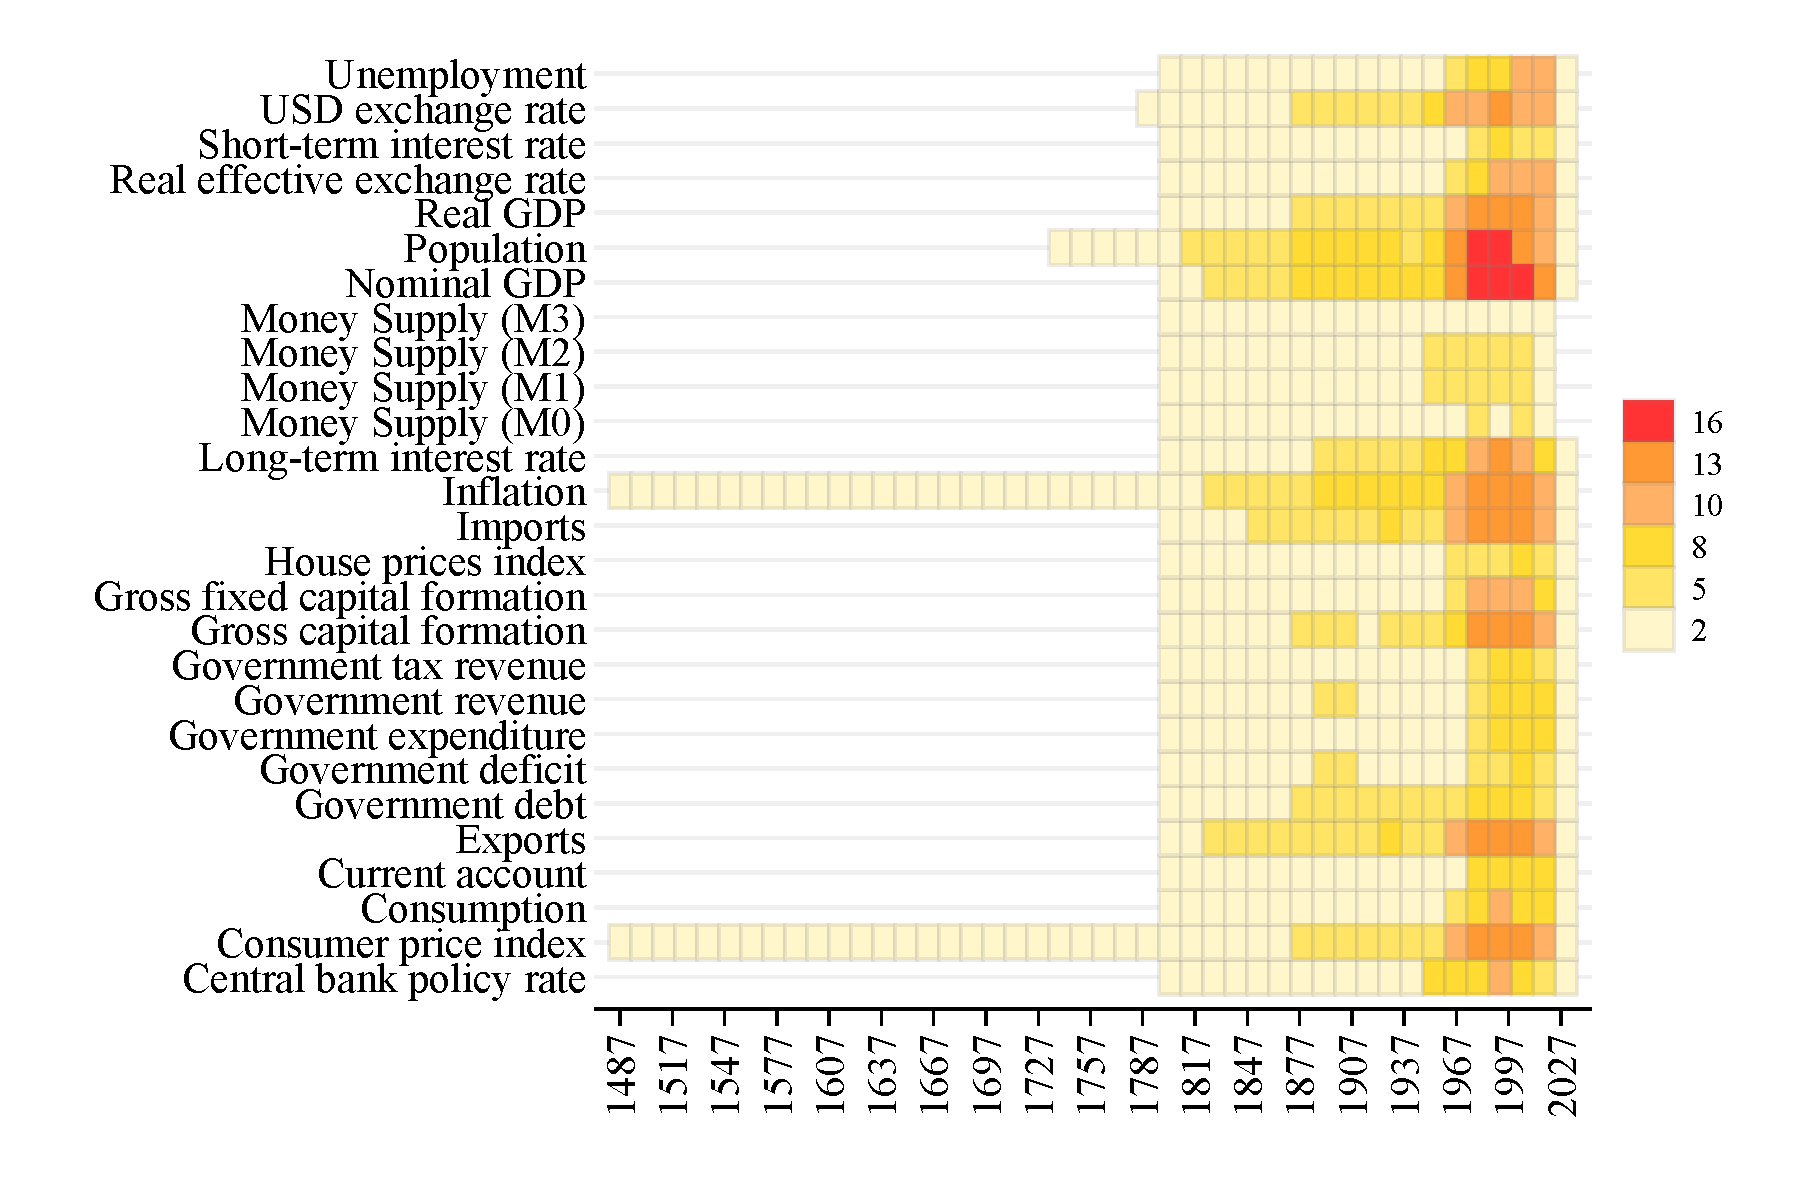
\includegraphics[width=\textwidth,height=0.8\textheight,keepaspectratio]{graphs/DNK_heatmap.pdf}
\end{figure}
\setcounter{page}{3}
\begin{adjustbox}{max totalsize={\paperwidth}{\paperheight},center}
\begin{minipage}[t][\textheight][t]{\textwidth}
\vspace*{0.5cm}
\phantomsection
\addcontentsline{toc}{section}{Current account balance}
\begin{center}
{\Large\bfseries Current account balance}
\end{center}
\vspace{0.5cm}
\begin{table}[H]
\centering
\small
\begin{tabular}{|l|l|l|}
\hline
\textbf{Source} & \textbf{Time span} & \textbf{Notes} \\
\hline
\rowcolor{white}\cite{JST}& 1874 - 1974 &Spliced using overlapping data in 1975. \\
\rowcolor{lightgray}\cite{OECD_EO}& 1975 - 2025 &Baseline source, overlaps with base year 2018. \\
\rowcolor{white}\cite{IMF_WEO_forecast}& 2026 - 2029 &Spliced using overlapping data in 2030. \\
\hline
\end{tabular}
\end{table}
\begin{figure}[H]
\centering
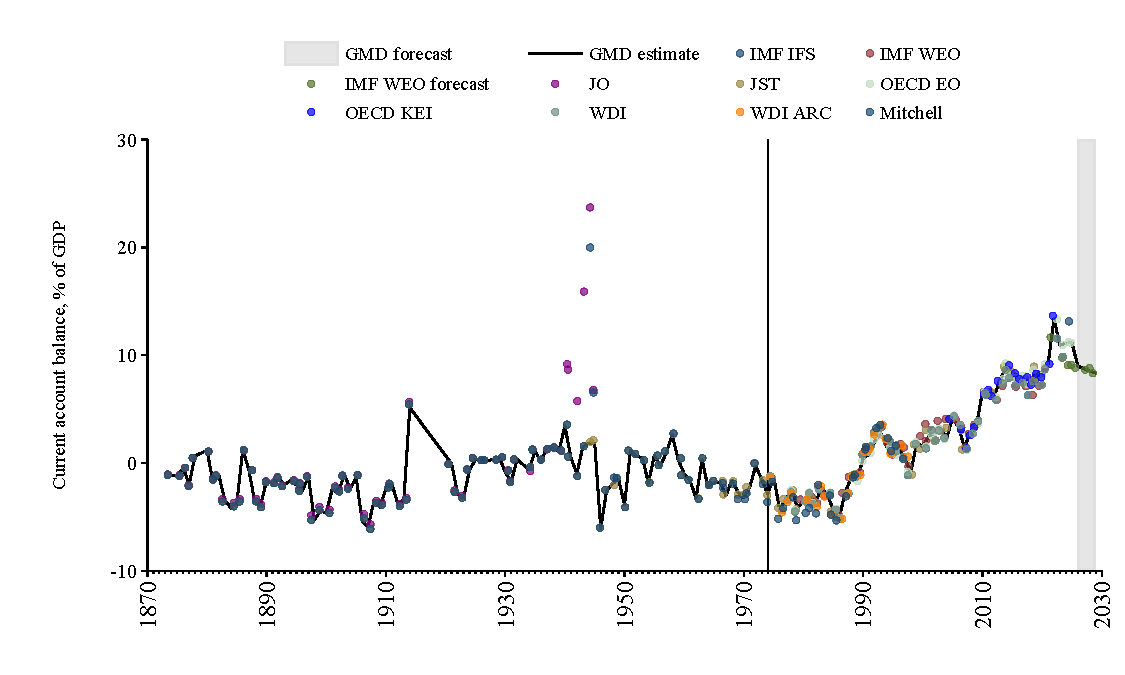
\includegraphics[width=\textwidth,height=0.6\textheight,keepaspectratio]{graphs/DNK_CA_GDP.pdf}
\end{figure}
\end{minipage}
\end{adjustbox}
\begin{adjustbox}{max totalsize={\paperwidth}{\paperheight},center}
\begin{minipage}[t][\textheight][t]{\textwidth}
\vspace*{0.5cm}
\phantomsection
\addcontentsline{toc}{section}{Consumer price index}
\begin{center}
{\Large\bfseries Consumer price index}
\end{center}
\vspace{0.5cm}
\begin{table}[H]
\centering
\small
\begin{tabular}{|l|l|l|}
\hline
\textbf{Source} & \textbf{Time span} & \textbf{Notes} \\
\hline
\rowcolor{white}\cite{CS1_DNK}& 1487 - 1899 &Spliced using overlapping data in 1900: (ratio = 39.7\%). \\
\rowcolor{lightgray}\cite{BIS}& 1900 - 2024 &Baseline source, overlaps with base year 2018. \\
\rowcolor{white}\cite{AMECO}& 2025 - 2026 &Spliced using overlapping data in 2027: (ratio = 107.2\%). \\
\rowcolor{lightgray}\cite{IMF_WEO_forecast}& 2027 - 2029 &Spliced using overlapping data in 2030: (ratio = 105.6\%). \\
\hline
\end{tabular}
\end{table}
\begin{figure}[H]
\centering
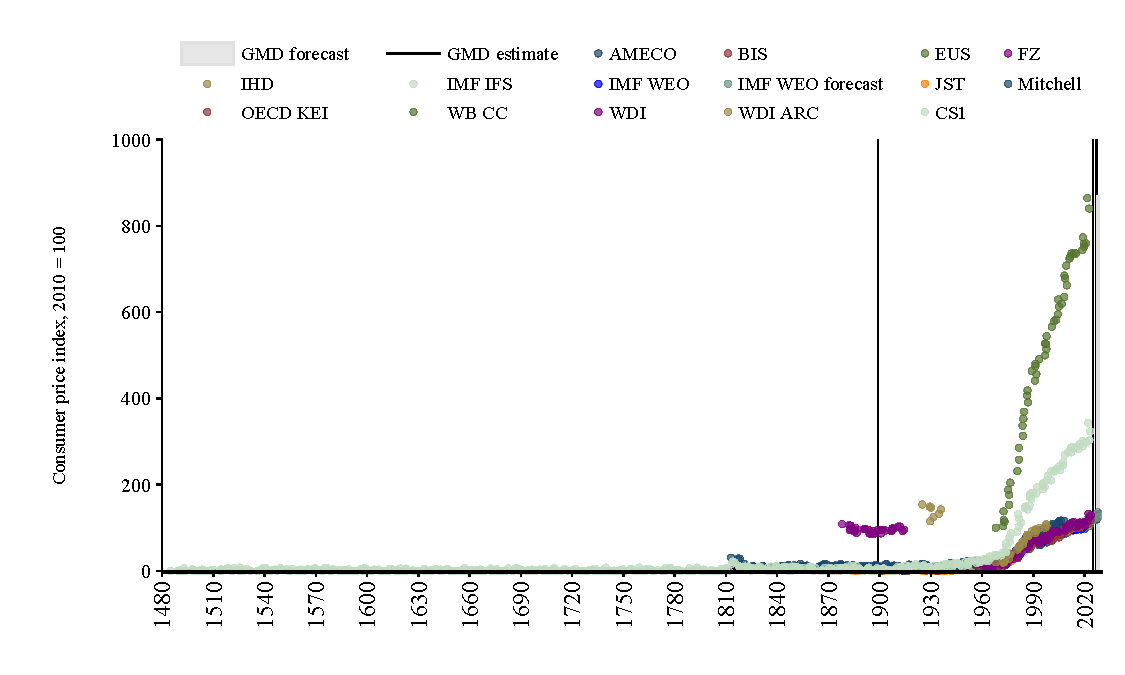
\includegraphics[width=\textwidth,height=0.6\textheight,keepaspectratio]{graphs/DNK_CPI.pdf}
\end{figure}
\end{minipage}
\end{adjustbox}
\begin{adjustbox}{max totalsize={\paperwidth}{\paperheight},center}
\begin{minipage}[t][\textheight][t]{\textwidth}
\vspace*{0.5cm}
\phantomsection
\addcontentsline{toc}{section}{House price index}
\begin{center}
{\Large\bfseries House price index}
\end{center}
\vspace{0.5cm}
\begin{table}[H]
\centering
\small
\begin{tabular}{|l|l|l|}
\hline
\textbf{Source} & \textbf{Time span} & \textbf{Notes} \\
\hline
\rowcolor{white}\cite{CS1_DNK}& 1860 - 1969 &Spliced using overlapping data in 1970. \\
\rowcolor{lightgray}\cite{BIS}& 1970 - 2024 &Baseline source, overlaps with base year 2018. \\
\hline
\end{tabular}
\end{table}
\begin{figure}[H]
\centering
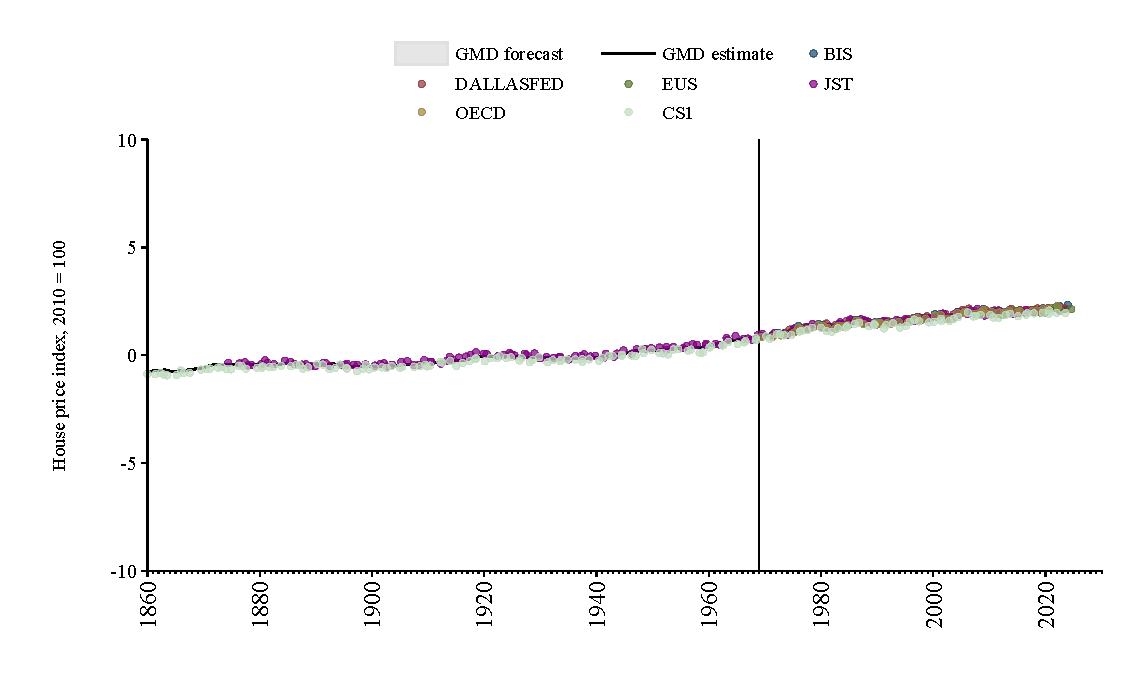
\includegraphics[width=\textwidth,height=0.6\textheight,keepaspectratio]{graphs/DNK_HPI.pdf}
\end{figure}
\end{minipage}
\end{adjustbox}
\begin{adjustbox}{max totalsize={\paperwidth}{\paperheight},center}
\begin{minipage}[t][\textheight][t]{\textwidth}
\vspace*{0.5cm}
\phantomsection
\addcontentsline{toc}{section}{Money supply (M0)}
\begin{center}
{\Large\bfseries Money supply (M0)}
\end{center}
\vspace{0.5cm}
\begin{table}[H]
\centering
\small
\begin{tabular}{|l|l|l|}
\hline
\textbf{Source} & \textbf{Time span} & \textbf{Notes} \\
\hline
\rowcolor{white}\cite{Mitchell}& 1819 - 1891 &Spliced using overlapping data in 1892: (ratio = 97\%). \\
\rowcolor{lightgray}\cite{FZ}& 1892 - 1892 &Spliced using overlapping data in 1893: (ratio = 60.2\%). \\
\rowcolor{white}\cite{Mitchell}& 1893 - 1949 &Spliced using overlapping data in 1950: (ratio = 96.7\%). \\
\rowcolor{lightgray}\cite{IMF_MFS}& 1950 - 2008 &Spliced using overlapping data in 2009: (ratio = 66.2\%). \\
\rowcolor{white}\cite{Mitchell}& 2009 - 2010 &Spliced using overlapping data in 2011. \\
\hline
\end{tabular}
\end{table}
\begin{figure}[H]
\centering
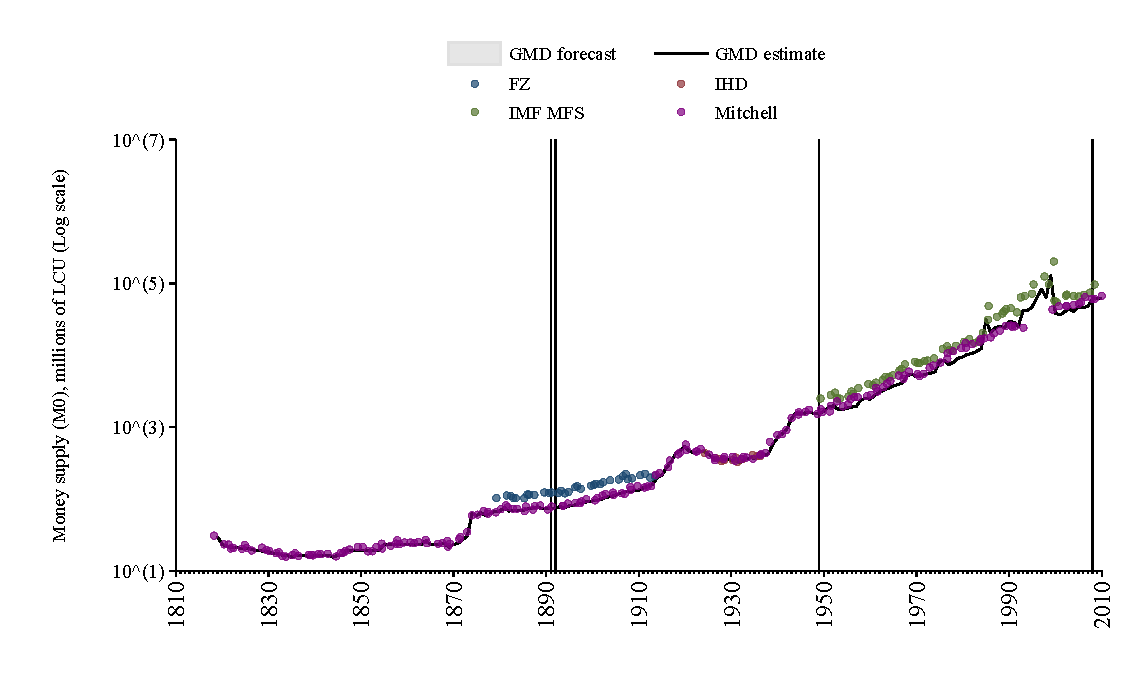
\includegraphics[width=\textwidth,height=0.6\textheight,keepaspectratio]{graphs/DNK_M0.pdf}
\end{figure}
\end{minipage}
\end{adjustbox}
\begin{adjustbox}{max totalsize={\paperwidth}{\paperheight},center}
\begin{minipage}[t][\textheight][t]{\textwidth}
\vspace*{0.5cm}
\phantomsection
\addcontentsline{toc}{section}{Money supply (M1)}
\begin{center}
{\Large\bfseries Money supply (M1)}
\end{center}
\vspace{0.5cm}
\begin{table}[H]
\centering
\small
\begin{tabular}{|l|l|l|}
\hline
\textbf{Source} & \textbf{Time span} & \textbf{Notes} \\
\hline
\rowcolor{white}\cite{JST}& 1870 - 1945 &Spliced using overlapping data in 1946: (ratio = 83.4\%). \\
\rowcolor{lightgray}\cite{IMF_MFS}& 1946 - 1990 &Spliced using overlapping data in 1991: (ratio = 91.3\%). \\
\rowcolor{white}\cite{OECD_MEI}& 1991 - 2023 &Baseline source, overlaps with base year 2018. \\
\hline
\end{tabular}
\end{table}
\begin{figure}[H]
\centering
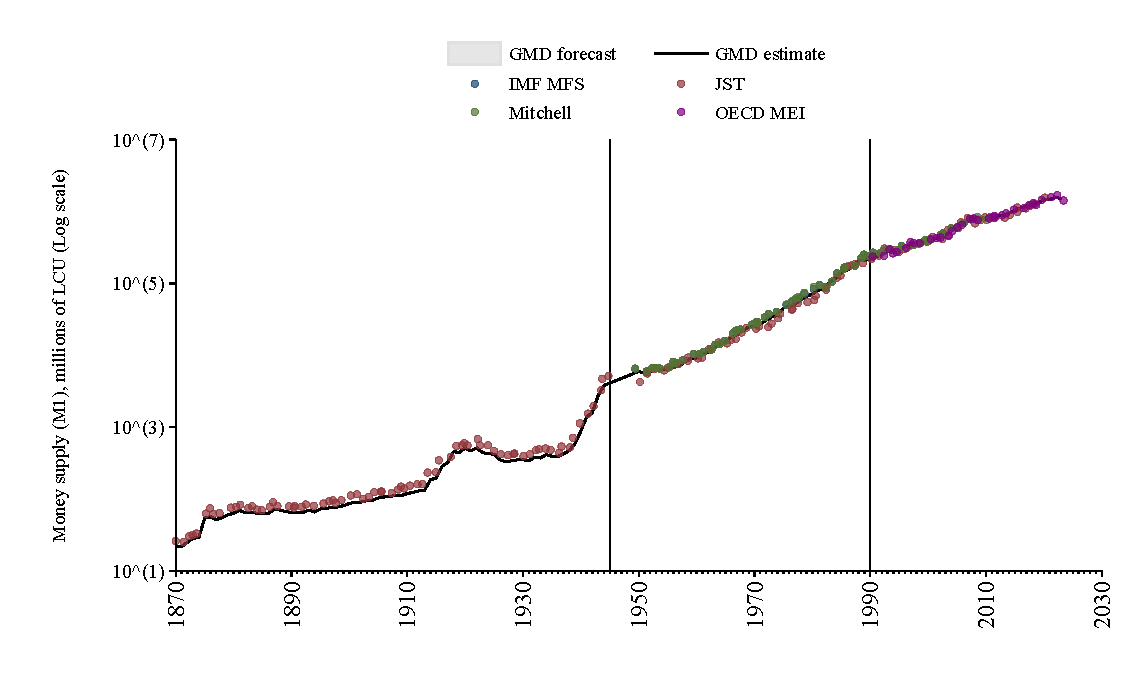
\includegraphics[width=\textwidth,height=0.6\textheight,keepaspectratio]{graphs/DNK_M1.pdf}
\end{figure}
\end{minipage}
\end{adjustbox}
\begin{adjustbox}{max totalsize={\paperwidth}{\paperheight},center}
\begin{minipage}[t][\textheight][t]{\textwidth}
\vspace*{0.5cm}
\phantomsection
\addcontentsline{toc}{section}{Money supply (M2)}
\begin{center}
{\Large\bfseries Money supply (M2)}
\end{center}
\vspace{0.5cm}
\begin{table}[H]
\centering
\small
\begin{tabular}{|l|l|l|}
\hline
\textbf{Source} & \textbf{Time span} & \textbf{Notes} \\
\hline
\rowcolor{white}\cite{JST}& 1870 - 1949 &Spliced using overlapping data in 1950: (ratio = 133.1\%). \\
\rowcolor{lightgray}\cite{IMF_MFS}& 1950 - 2008 &Spliced using overlapping data in 2009: (ratio = 95.2\%). \\
\rowcolor{white}\cite{JST}& 2009 - 2020 &Baseline source, overlaps with base year 2018. \\
\hline
\end{tabular}
\end{table}
\begin{figure}[H]
\centering
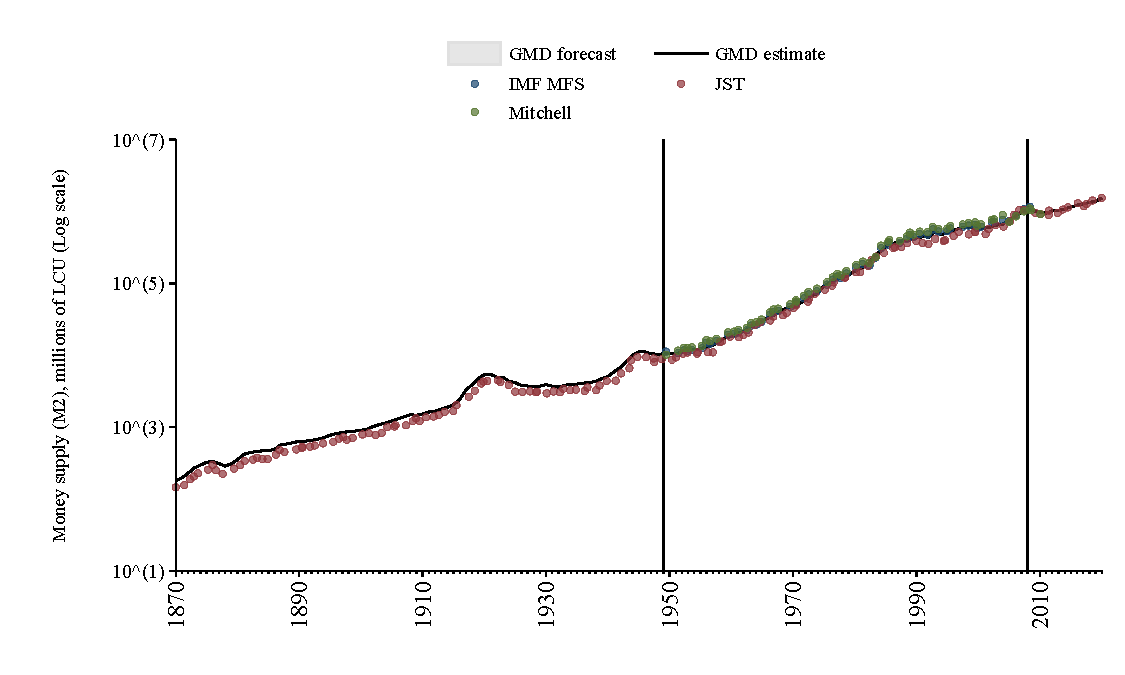
\includegraphics[width=\textwidth,height=0.6\textheight,keepaspectratio]{graphs/DNK_M2.pdf}
\end{figure}
\end{minipage}
\end{adjustbox}
\begin{adjustbox}{max totalsize={\paperwidth}{\paperheight},center}
\begin{minipage}[t][\textheight][t]{\textwidth}
\vspace*{0.5cm}
\phantomsection
\addcontentsline{toc}{section}{Money supply (M3)}
\begin{center}
{\Large\bfseries Money supply (M3)}
\end{center}
\vspace{0.5cm}
\begin{table}[H]
\centering
\small
\begin{tabular}{|l|l|l|}
\hline
\textbf{Source} & \textbf{Time span} & \textbf{Notes} \\
\hline
\rowcolor{white}\cite{OECD_MEI}& 1970 - 2023 &Baseline source, overlaps with base year 2018. \\
\hline
\end{tabular}
\end{table}
\begin{figure}[H]
\centering
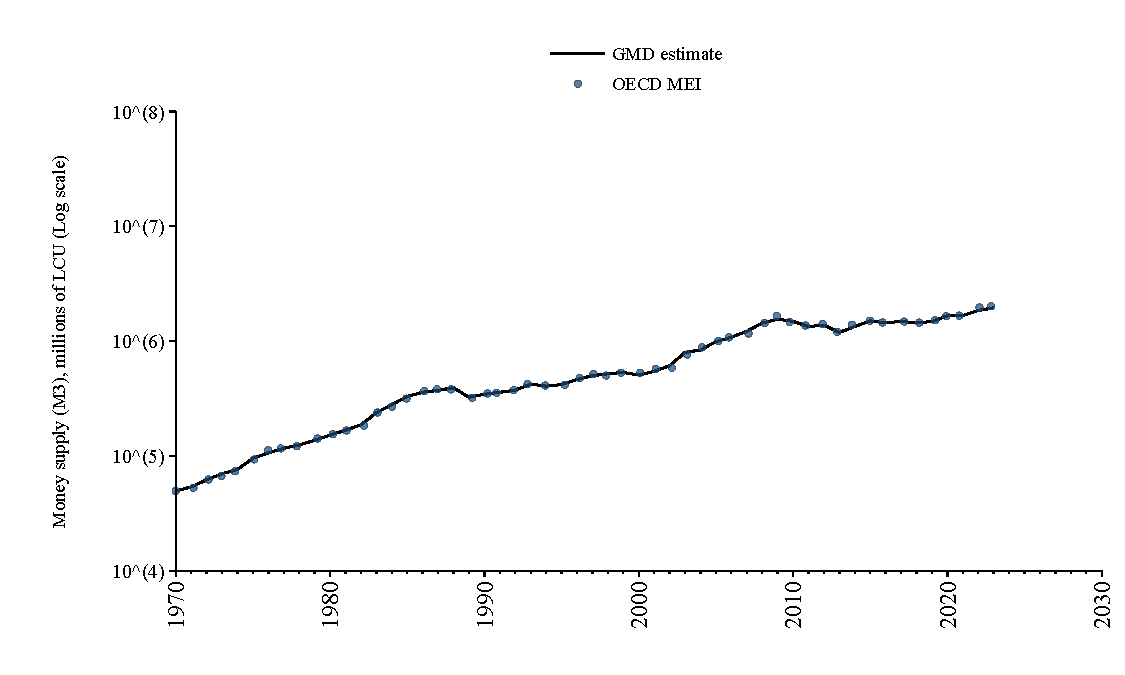
\includegraphics[width=\textwidth,height=0.6\textheight,keepaspectratio]{graphs/DNK_M3.pdf}
\end{figure}
\end{minipage}
\end{adjustbox}
\begin{adjustbox}{max totalsize={\paperwidth}{\paperheight},center}
\begin{minipage}[t][\textheight][t]{\textwidth}
\vspace*{0.5cm}
\phantomsection
\addcontentsline{toc}{section}{Real effective exchange rate}
\begin{center}
{\Large\bfseries Real effective exchange rate}
\end{center}
\vspace{0.5cm}
\begin{table}[H]
\centering
\small
\begin{tabular}{|l|l|l|}
\hline
\textbf{Source} & \textbf{Time span} & \textbf{Notes} \\
\hline
\rowcolor{white}\cite{LUND}& 1870 - 1959 &Spliced using overlapping data in 1960: (ratio = 65.1\%). \\
\rowcolor{lightgray}\cite{BRUEGEL}& 1960 - 1974 &Spliced using overlapping data in 1975: (ratio = 103.5\%). \\
\rowcolor{white}\cite{WDI_ARC}& 1975 - 1978 &Spliced using overlapping data in 1979: (ratio = 97.7\%). \\
\rowcolor{lightgray}\cite{WDI}& 1979 - 2023 &Baseline source, overlaps with base year 2018. \\
\rowcolor{white}\cite{BIS}& 2024 - 2025 &Spliced using overlapping data in 2026: (ratio = 98.5\%). \\
\hline
\end{tabular}
\end{table}
\begin{figure}[H]
\centering
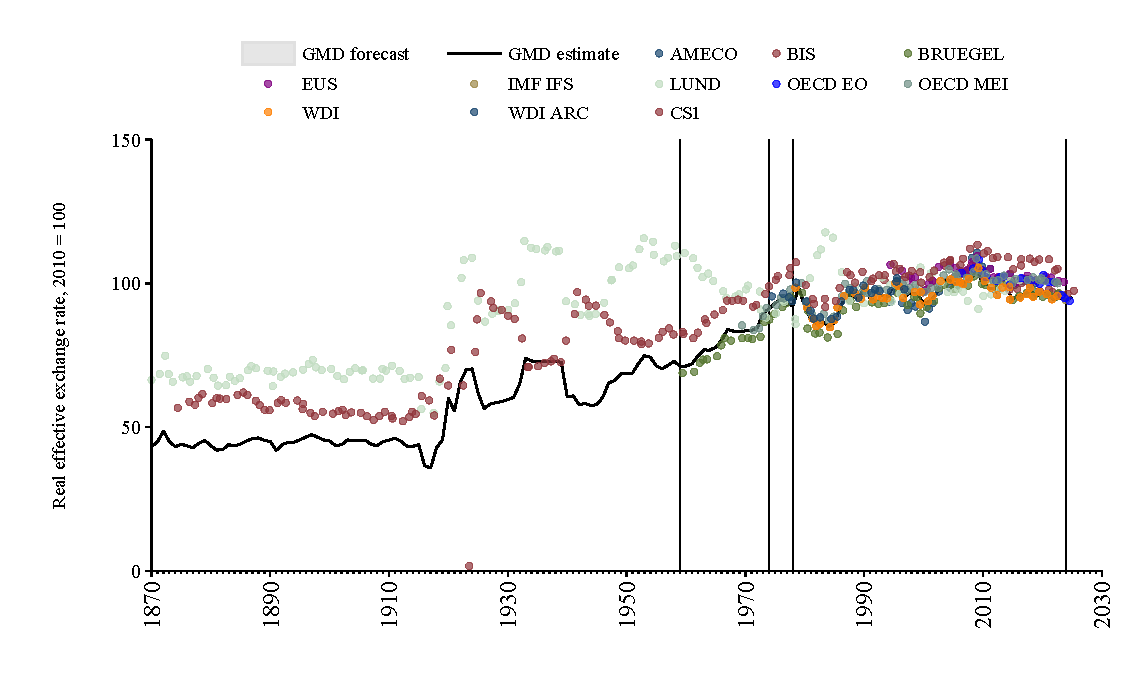
\includegraphics[width=\textwidth,height=0.6\textheight,keepaspectratio]{graphs/DNK_REER.pdf}
\end{figure}
\end{minipage}
\end{adjustbox}
\begin{adjustbox}{max totalsize={\paperwidth}{\paperheight},center}
\begin{minipage}[t][\textheight][t]{\textwidth}
\vspace*{0.5cm}
\phantomsection
\addcontentsline{toc}{section}{USD exchange rate}
\begin{center}
{\Large\bfseries USD exchange rate}
\end{center}
\vspace{0.5cm}
\begin{table}[H]
\centering
\small
\begin{tabular}{|l|l|l|}
\hline
\textbf{Source} & \textbf{Time span} & \textbf{Notes} \\
\hline
\rowcolor{white}\cite{CS1_DNK}& 1791 - 1949 &Spliced using overlapping data in 1950. \\
\rowcolor{lightgray}\cite{IMF_IFS}& 1950 - 1952 &Spliced using overlapping data in 1953. \\
\rowcolor{white}\cite{BIS}& 1953 - 2024 &Baseline source, overlaps with base year 2018. \\
\rowcolor{lightgray}\cite{OECD_EO}& 2025 - 2025 &Spliced using overlapping data in 2026. \\
\hline
\end{tabular}
\end{table}
\begin{figure}[H]
\centering
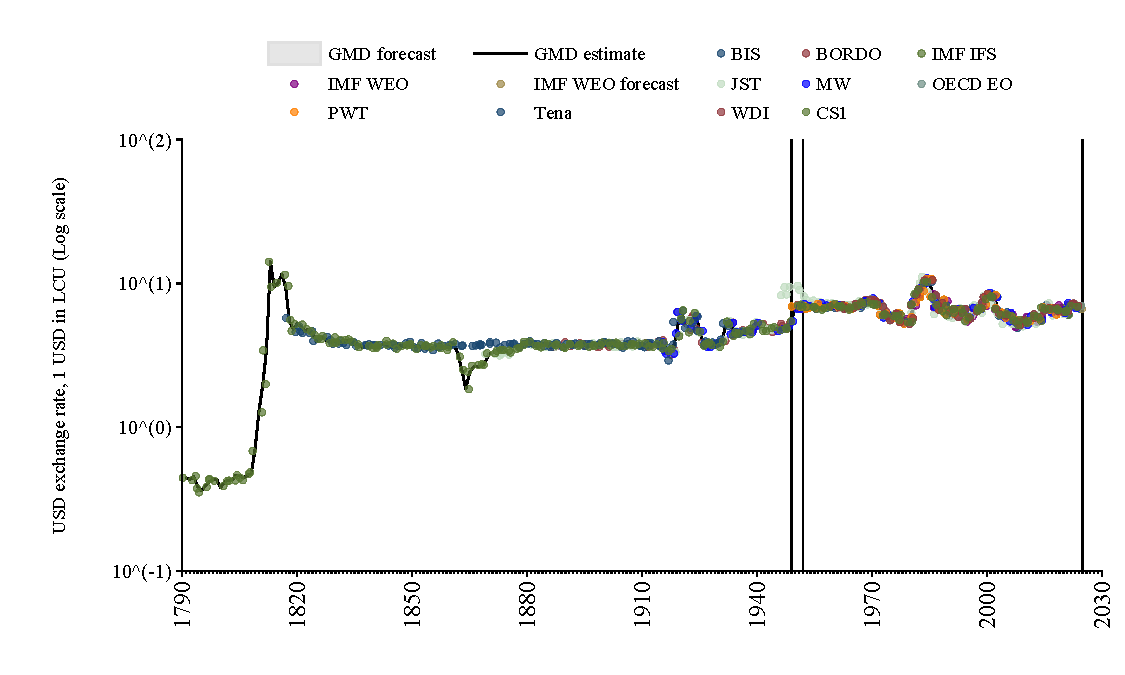
\includegraphics[width=\textwidth,height=0.6\textheight,keepaspectratio]{graphs/DNK_USDfx.pdf}
\end{figure}
\end{minipage}
\end{adjustbox}
\begin{adjustbox}{max totalsize={\paperwidth}{\paperheight},center}
\begin{minipage}[t][\textheight][t]{\textwidth}
\vspace*{0.5cm}
\phantomsection
\addcontentsline{toc}{section}{Central bank policy rate}
\begin{center}
{\Large\bfseries Central bank policy rate}
\end{center}
\vspace{0.5cm}
\begin{table}[H]
\centering
\small
\begin{tabular}{|l|l|l|}
\hline
\textbf{Source} & \textbf{Time span} & \textbf{Notes} \\
\hline
\rowcolor{white}\cite{CS1_DNK}& 1819 - 1945 &Spliced using overlapping data in 1946. \\
\rowcolor{lightgray}\cite{BIS}& 1946 - 2025 &Baseline source, overlaps with base year 2018. \\
\hline
\end{tabular}
\end{table}
\begin{figure}[H]
\centering
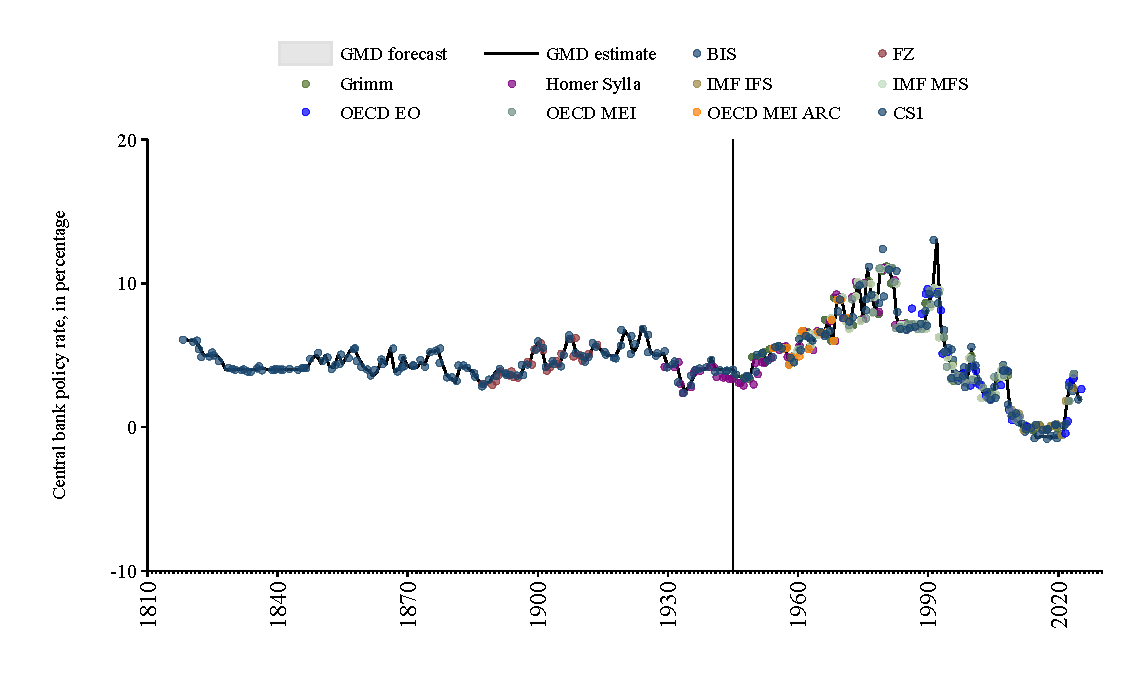
\includegraphics[width=\textwidth,height=0.6\textheight,keepaspectratio]{graphs/DNK_cbrate.pdf}
\end{figure}
\end{minipage}
\end{adjustbox}
\begin{adjustbox}{max totalsize={\paperwidth}{\paperheight},center}
\begin{minipage}[t][\textheight][t]{\textwidth}
\vspace*{0.5cm}
\phantomsection
\addcontentsline{toc}{section}{Total consumption}
\begin{center}
{\Large\bfseries Total consumption}
\end{center}
\vspace{0.5cm}
\begin{table}[H]
\centering
\small
\begin{tabular}{|l|l|l|}
\hline
\textbf{Source} & \textbf{Time span} & \textbf{Notes} \\
\hline
\rowcolor{white}\cite{CS1_DNK}& 1844 - 1959 &Spliced using overlapping data in 1960: (ratio = 100.2\%). \\
\rowcolor{lightgray}\cite{AMECO}& 1960 - 1965 &Spliced using overlapping data in 1966. \\
\rowcolor{white}\cite{OECD_EO}& 1966 - 2025 &Baseline source, overlaps with base year 2018. \\
\rowcolor{lightgray}\cite{AMECO}& 2026 - 2026 &Spliced using overlapping data in 2027: (ratio = 98.6\%). \\
\hline
\end{tabular}
\end{table}
\begin{figure}[H]
\centering
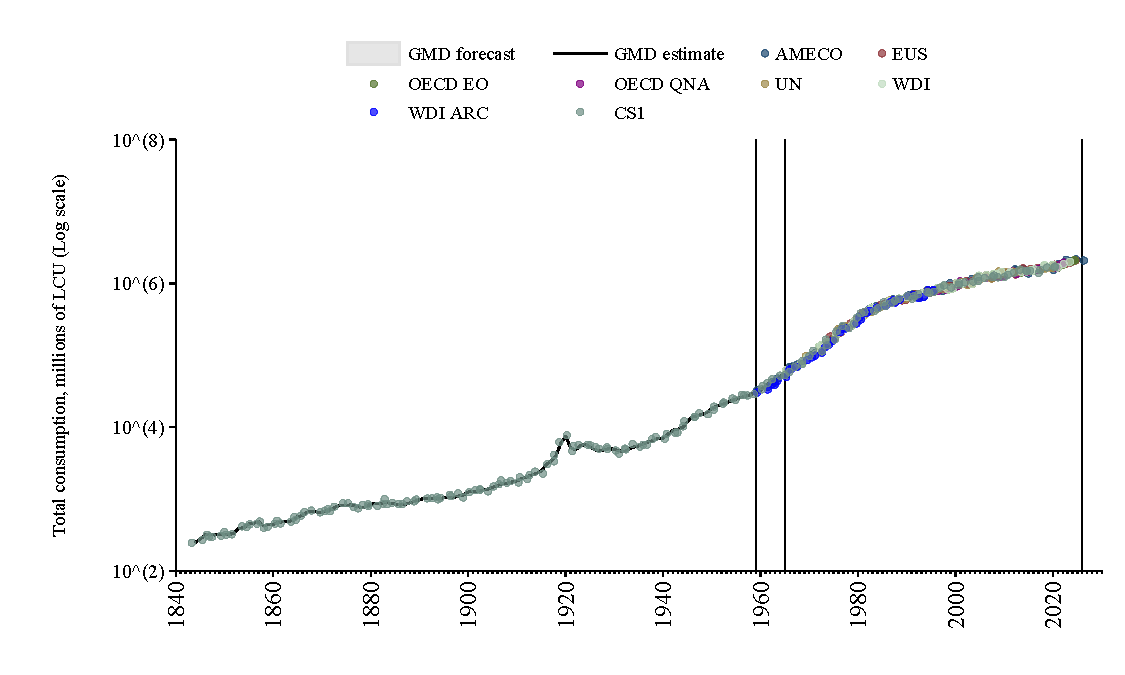
\includegraphics[width=\textwidth,height=0.6\textheight,keepaspectratio]{graphs/DNK_cons.pdf}
\end{figure}
\end{minipage}
\end{adjustbox}
\begin{adjustbox}{max totalsize={\paperwidth}{\paperheight},center}
\begin{minipage}[t][\textheight][t]{\textwidth}
\vspace*{0.5cm}
\phantomsection
\addcontentsline{toc}{section}{Total consumption to GDP ratio}
\begin{center}
{\Large\bfseries Total consumption to GDP ratio}
\end{center}
\vspace{0.5cm}
\begin{table}[H]
\centering
\small
\begin{tabular}{|l|l|l|}
\hline
\textbf{Source} & \textbf{Time span} & \textbf{Notes} \\
\hline
\rowcolor{white}\cite{CS1_DNK}& 1844 - 1959 &Spliced using overlapping data in 1960: (ratio = 97.2\%). \\
\rowcolor{lightgray}\cite{WDI_ARC}& 1960 - 1965 &Spliced using overlapping data in 1966: (ratio = 102.9\%). \\
\rowcolor{white}\cite{WDI}& 1966 - 2023 &Baseline source, overlaps with base year 2018. \\
\rowcolor{lightgray}\cite{EUS}& 2024 - 2024 &Spliced using overlapping data in 2025. \\
\rowcolor{white}\cite{OECD_EO}& 2025 - 2025 &Spliced using overlapping data in 2026: (ratio = 98\%). \\
\rowcolor{lightgray}\cite{AMECO}& 2026 - 2026 &Spliced using overlapping data in 2027: (ratio = 97.9\%). \\
\hline
\end{tabular}
\end{table}
\begin{figure}[H]
\centering
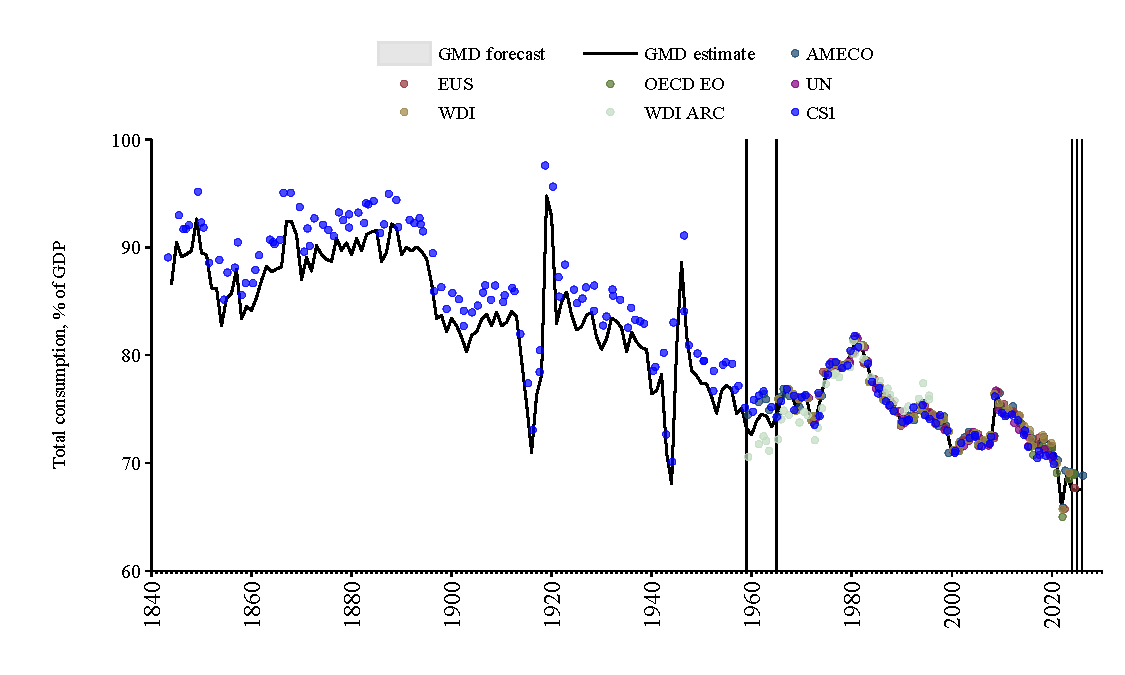
\includegraphics[width=\textwidth,height=0.6\textheight,keepaspectratio]{graphs/DNK_cons_GDP.pdf}
\end{figure}
\end{minipage}
\end{adjustbox}
\begin{adjustbox}{max totalsize={\paperwidth}{\paperheight},center}
\begin{minipage}[t][\textheight][t]{\textwidth}
\vspace*{0.5cm}
\phantomsection
\addcontentsline{toc}{section}{Exports}
\begin{center}
{\Large\bfseries Exports}
\end{center}
\vspace{0.5cm}
\begin{table}[H]
\centering
\small
\begin{tabular}{|l|l|l|}
\hline
\textbf{Source} & \textbf{Time span} & \textbf{Notes} \\
\hline
\rowcolor{white}\cite{CS1_DNK}& 1817 - 1959 &Spliced using overlapping data in 1960: (ratio = 100.2\%). \\
\rowcolor{lightgray}\cite{AMECO}& 1960 - 1965 &Spliced using overlapping data in 1966: (ratio = 100.1\%). \\
\rowcolor{white}\cite{OECD_EO}& 1966 - 2025 &Baseline source, overlaps with base year 2018. \\
\rowcolor{lightgray}\cite{AMECO}& 2026 - 2026 &Spliced using overlapping data in 2027: (ratio = 104.3\%). \\
\rowcolor{white}\cite{IMF_WEO_forecast}& 2027 - 2029 &Spliced using overlapping data in 2030: (ratio = 102.6\%). \\
\hline
\end{tabular}
\end{table}
\begin{figure}[H]
\centering
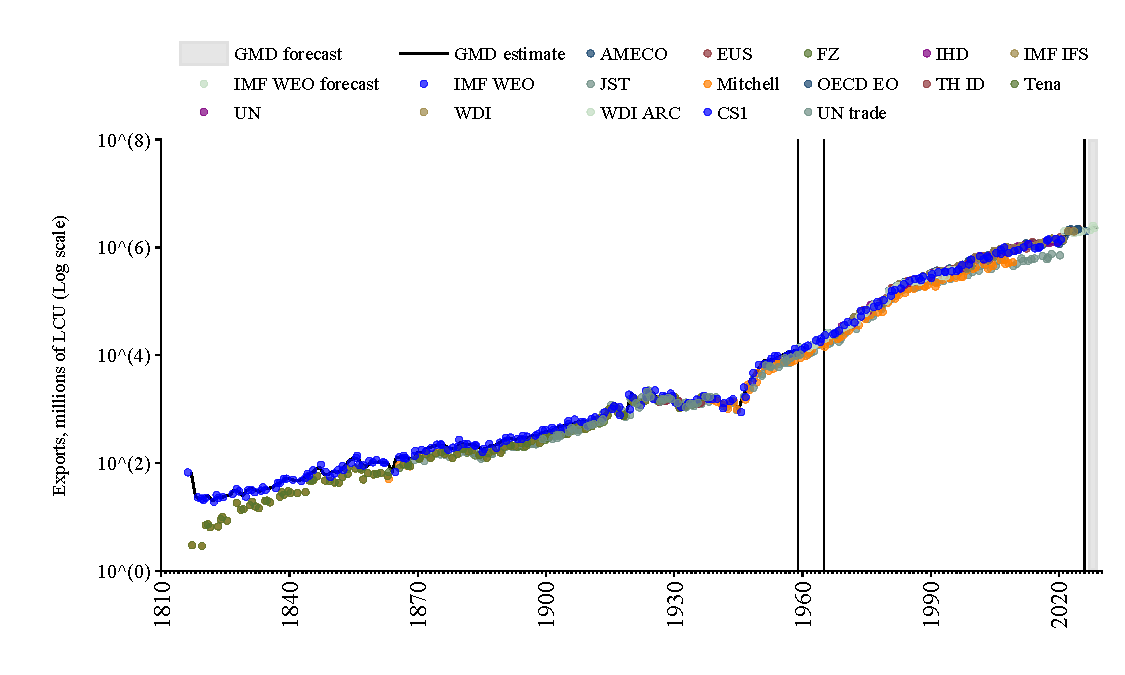
\includegraphics[width=\textwidth,height=0.6\textheight,keepaspectratio]{graphs/DNK_exports.pdf}
\end{figure}
\end{minipage}
\end{adjustbox}
\begin{adjustbox}{max totalsize={\paperwidth}{\paperheight},center}
\begin{minipage}[t][\textheight][t]{\textwidth}
\vspace*{0.5cm}
\phantomsection
\addcontentsline{toc}{section}{Exports to GDP ratio}
\begin{center}
{\Large\bfseries Exports to GDP ratio}
\end{center}
\vspace{0.5cm}
\begin{table}[H]
\centering
\small
\begin{tabular}{|l|l|l|}
\hline
\textbf{Source} & \textbf{Time span} & \textbf{Notes} \\
\hline
\rowcolor{white}\cite{CS1_DNK}& 1817 - 1869 &Spliced using overlapping data in 1870: (ratio = 107.4\%). \\
\rowcolor{lightgray}\cite{JST}& 1870 - 1965 &Spliced using overlapping data in 1966: (ratio = 136.6\%). \\
\rowcolor{white}\cite{OECD_EO}& 1966 - 2025 &Baseline source, overlaps with base year 2018. \\
\rowcolor{lightgray}\cite{AMECO}& 2026 - 2026 &Spliced using overlapping data in 2027: (ratio = 105.8\%). \\
\rowcolor{white}\cite{IMF_WEO_forecast}& 2027 - 2029 &Spliced using overlapping data in 2030: (ratio = 100.7\%). \\
\hline
\end{tabular}
\end{table}
\begin{figure}[H]
\centering
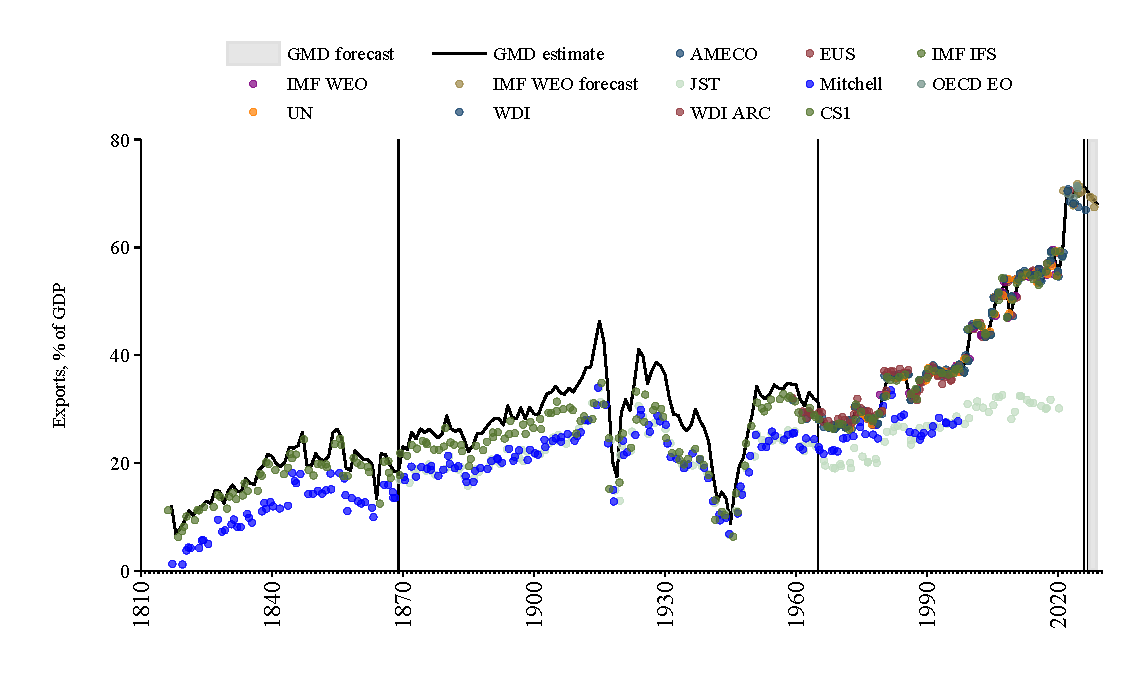
\includegraphics[width=\textwidth,height=0.6\textheight,keepaspectratio]{graphs/DNK_exports_GDP.pdf}
\end{figure}
\end{minipage}
\end{adjustbox}
\begin{adjustbox}{max totalsize={\paperwidth}{\paperheight},center}
\begin{minipage}[t][\textheight][t]{\textwidth}
\vspace*{0.5cm}
\phantomsection
\addcontentsline{toc}{section}{Fixed investment}
\begin{center}
{\Large\bfseries Fixed investment}
\end{center}
\vspace{0.5cm}
\begin{table}[H]
\centering
\small
\begin{tabular}{|l|l|l|}
\hline
\textbf{Source} & \textbf{Time span} & \textbf{Notes} \\
\hline
\rowcolor{white}\cite{JO}& 1850 - 1945 &Spliced using overlapping data in 1946: (ratio = 99.9\%). \\
\rowcolor{lightgray}\cite{AMECO}& 1946 - 1965 &Spliced using overlapping data in 1966. \\
\rowcolor{white}\cite{OECD_EO}& 1966 - 2025 &Baseline source, overlaps with base year 2018. \\
\rowcolor{lightgray}\cite{AMECO}& 2026 - 2026 &Spliced using overlapping data in 2027: (ratio = 92.4\%). \\
\hline
\end{tabular}
\end{table}
\begin{figure}[H]
\centering
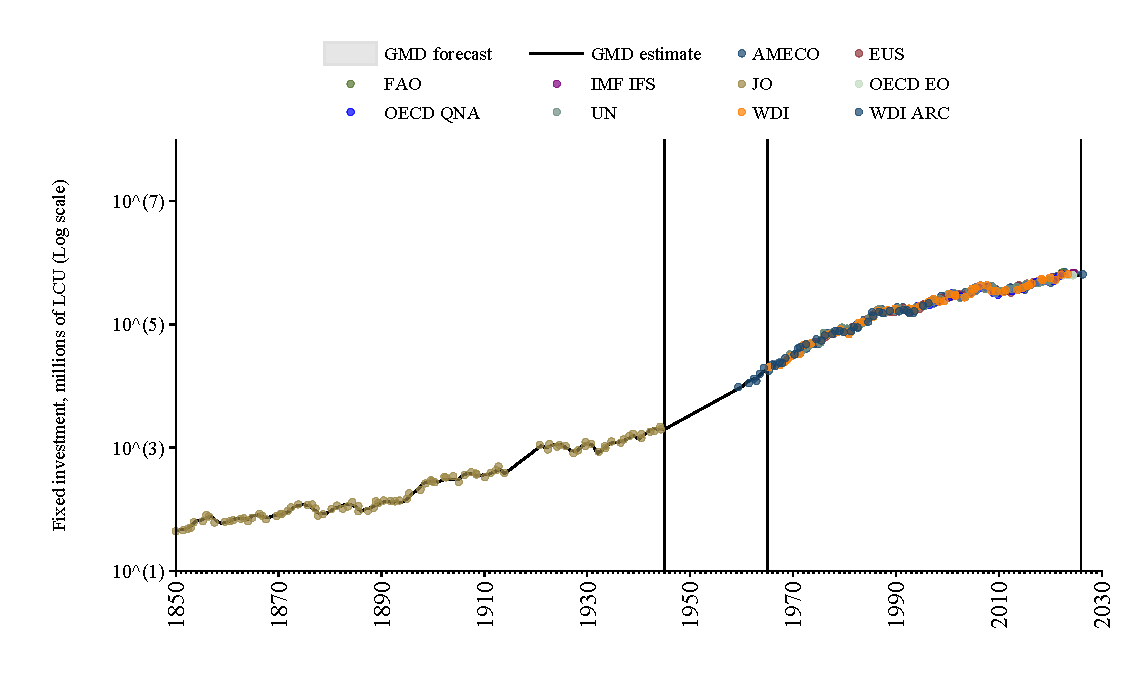
\includegraphics[width=\textwidth,height=0.6\textheight,keepaspectratio]{graphs/DNK_finv.pdf}
\end{figure}
\end{minipage}
\end{adjustbox}
\begin{adjustbox}{max totalsize={\paperwidth}{\paperheight},center}
\begin{minipage}[t][\textheight][t]{\textwidth}
\vspace*{0.5cm}
\phantomsection
\addcontentsline{toc}{section}{Fixed investment to GDP ratio}
\begin{center}
{\Large\bfseries Fixed investment to GDP ratio}
\end{center}
\vspace{0.5cm}
\begin{table}[H]
\centering
\small
\begin{tabular}{|l|l|l|}
\hline
\textbf{Source} & \textbf{Time span} & \textbf{Notes} \\
\hline
\rowcolor{white}\cite{JO}& 1850 - 1945 &Spliced using overlapping data in 1946. \\
\rowcolor{lightgray}\cite{AMECO}& 1946 - 1964 &Spliced using overlapping data in 1965. \\
\rowcolor{white}\cite{WDI_ARC}& 1965 - 1965 &Spliced using overlapping data in 1966: (ratio = 89.9\%). \\
\rowcolor{lightgray}\cite{WDI}& 1966 - 1974 &Spliced using overlapping data in 1975. \\
\rowcolor{white}\cite{EUS}& 1975 - 2024 &Baseline source, overlaps with base year 2018. \\
\rowcolor{lightgray}\cite{OECD_EO}& 2025 - 2025 &Spliced using overlapping data in 2026: (ratio = 108\%). \\
\rowcolor{white}\cite{AMECO}& 2026 - 2026 &Spliced using overlapping data in 2027: (ratio = 101.3\%). \\
\hline
\end{tabular}
\end{table}
\begin{figure}[H]
\centering
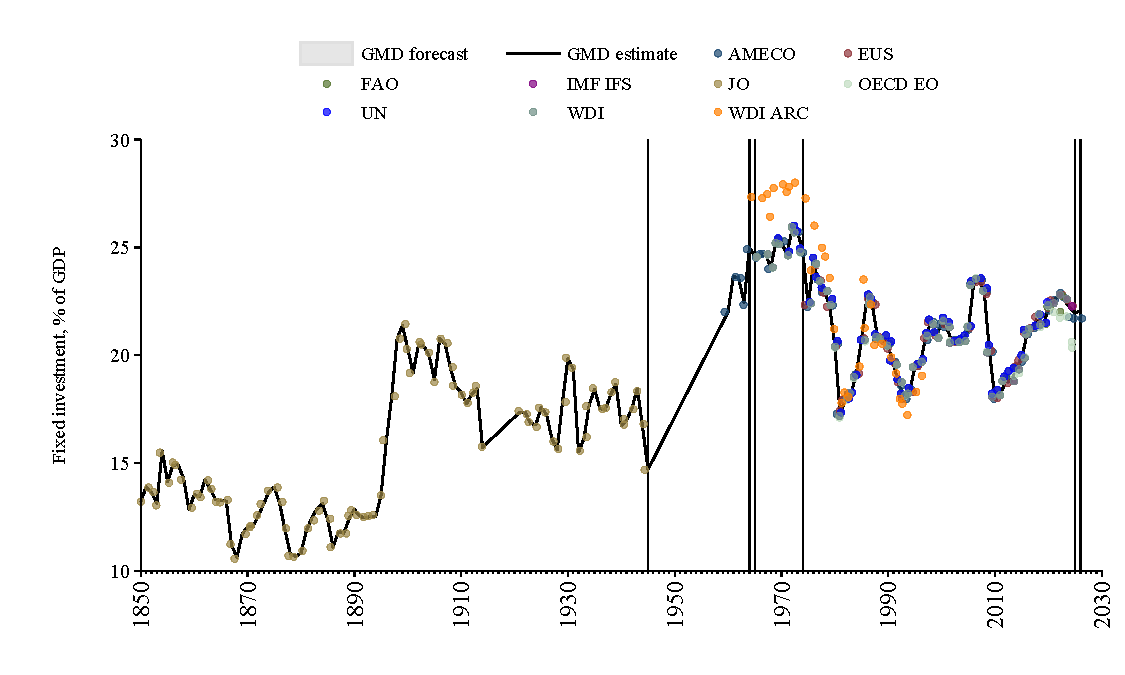
\includegraphics[width=\textwidth,height=0.6\textheight,keepaspectratio]{graphs/DNK_finv_GDP.pdf}
\end{figure}
\end{minipage}
\end{adjustbox}
\begin{adjustbox}{max totalsize={\paperwidth}{\paperheight},center}
\begin{minipage}[t][\textheight][t]{\textwidth}
\vspace*{0.5cm}
\phantomsection
\addcontentsline{toc}{section}{Government debt}
\begin{center}
{\Large\bfseries Government debt}
\end{center}
\vspace{0.5cm}
\begin{table}[H]
\centering
\small
\begin{tabular}{|l|l|l|}
\hline
\textbf{Source} & \textbf{Time span} & \textbf{Notes} \\
\hline
\rowcolor{white}\cite{IMF_FPP}& 1880 - 1946 &Spliced using overlapping data in 1947. Data refers to general government.\\
\rowcolor{lightgray}\cite{RR_debt}& 1947 - 1949 &Spliced using overlapping data in 1950. \\
\rowcolor{white}\cite{IMF_GDD}& 1950 - 2018 &Spliced using overlapping data in 2019. Data refers to central government.\\
\rowcolor{lightgray}\cite{IMF_FPP}& 2019 - 2023 &Spliced using overlapping data in 2024. Data refers to general government.\\
\rowcolor{white}\cite{OECD_EO}& 2024 - 2025 &Spliced using overlapping data in 2026. Data refers to general government.\\
\rowcolor{lightgray}\cite{IMF_WEO_forecast}& 2026 - 2029 &Spliced using overlapping data in 2030. \\
\hline
\end{tabular}
\end{table}
\begin{figure}[H]
\centering
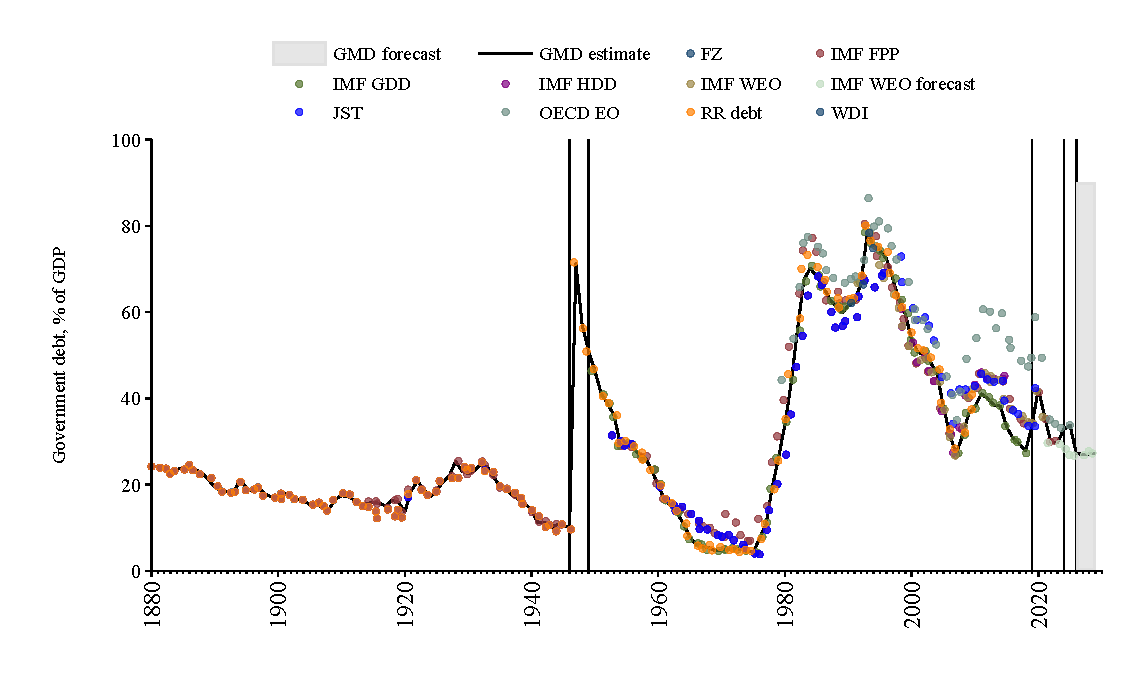
\includegraphics[width=\textwidth,height=0.6\textheight,keepaspectratio]{graphs/DNK_govdebt_GDP.pdf}
\end{figure}
\end{minipage}
\end{adjustbox}
\begin{adjustbox}{max totalsize={\paperwidth}{\paperheight},center}
\begin{minipage}[t][\textheight][t]{\textwidth}
\vspace*{0.5cm}
\phantomsection
\addcontentsline{toc}{section}{Government deficit}
\begin{center}
{\Large\bfseries Government deficit}
\end{center}
\vspace{0.5cm}
\begin{table}[H]
\centering
\small
\begin{tabular}{|l|l|l|}
\hline
\textbf{Source} & \textbf{Time span} & \textbf{Notes} \\
\hline
\rowcolor{white}\cite{Mitchell}& 1854 - 1879 &Spliced using overlapping data in 1880. \\
\rowcolor{lightgray}\cite{IMF_FPP}& 1880 - 1938 &Spliced using overlapping data in 1939. \\
\rowcolor{white}\cite{Mitchell}& 1939 - 1944 &Spliced using overlapping data in 1945. \\
\rowcolor{lightgray}\cite{IMF_FPP}& 1945 - 1945 &Spliced using overlapping data in 1946. \\
\rowcolor{white}\cite{Mitchell}& 1946 - 1953 &Spliced using overlapping data in 1954. \\
\rowcolor{lightgray}\cite{IMF_FPP}& 1954 - 1979 &Spliced using overlapping data in 1980. \\
\rowcolor{white}\cite{IMF_WEO}& 1980 - 1994 &Spliced using overlapping data in 1995. \\
\rowcolor{lightgray}\cite{EUS}& 1995 - 2024 &Baseline source, overlaps with base year 2018. \\
\rowcolor{white}\cite{IMF_WEO_forecast}& 2025 - 2029 &Spliced using overlapping data in 2030. \\
\hline
\end{tabular}
\end{table}
\begin{figure}[H]
\centering
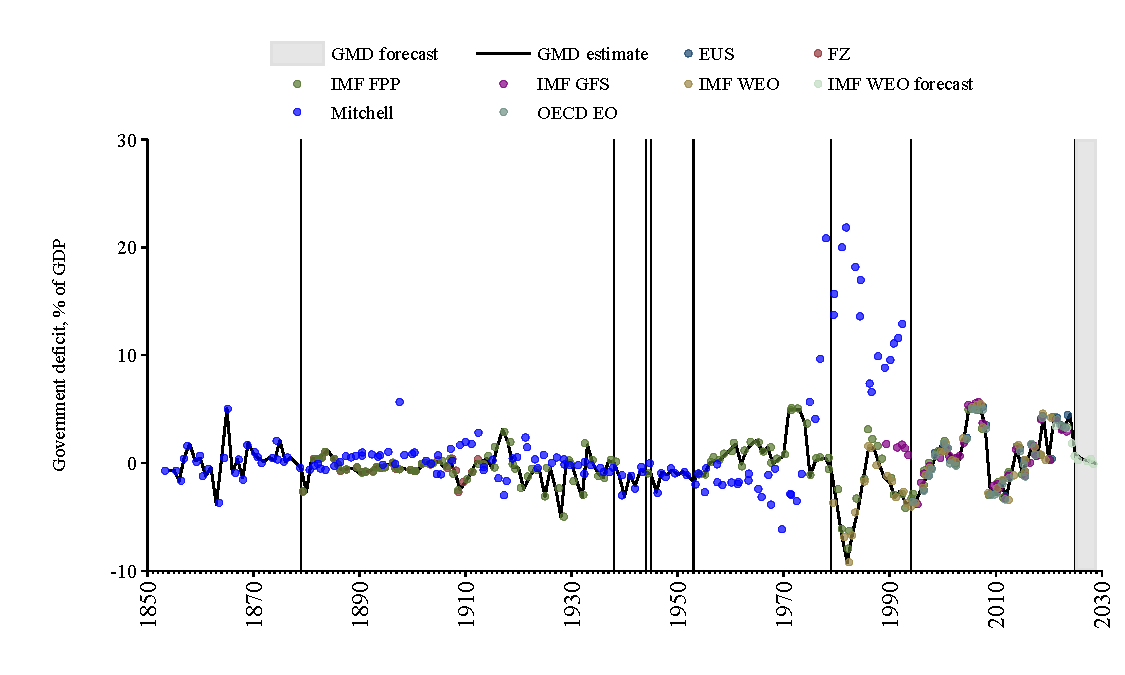
\includegraphics[width=\textwidth,height=0.6\textheight,keepaspectratio]{graphs/DNK_govdef_GDP.pdf}
\end{figure}
\end{minipage}
\end{adjustbox}
\begin{adjustbox}{max totalsize={\paperwidth}{\paperheight},center}
\begin{minipage}[t][\textheight][t]{\textwidth}
\vspace*{0.5cm}
\phantomsection
\addcontentsline{toc}{section}{Government expenditure}
\begin{center}
{\Large\bfseries Government expenditure}
\end{center}
\vspace{0.5cm}
\begin{table}[H]
\centering
\small
\begin{tabular}{|l|l|l|}
\hline
\textbf{Source} & \textbf{Time span} & \textbf{Notes} \\
\hline
\rowcolor{white}\cite{GMD_estimated}& 1854 - 2029 &Baseline source, overlaps with base year 2018. \\
\hline
\end{tabular}
\end{table}
\begin{figure}[H]
\centering
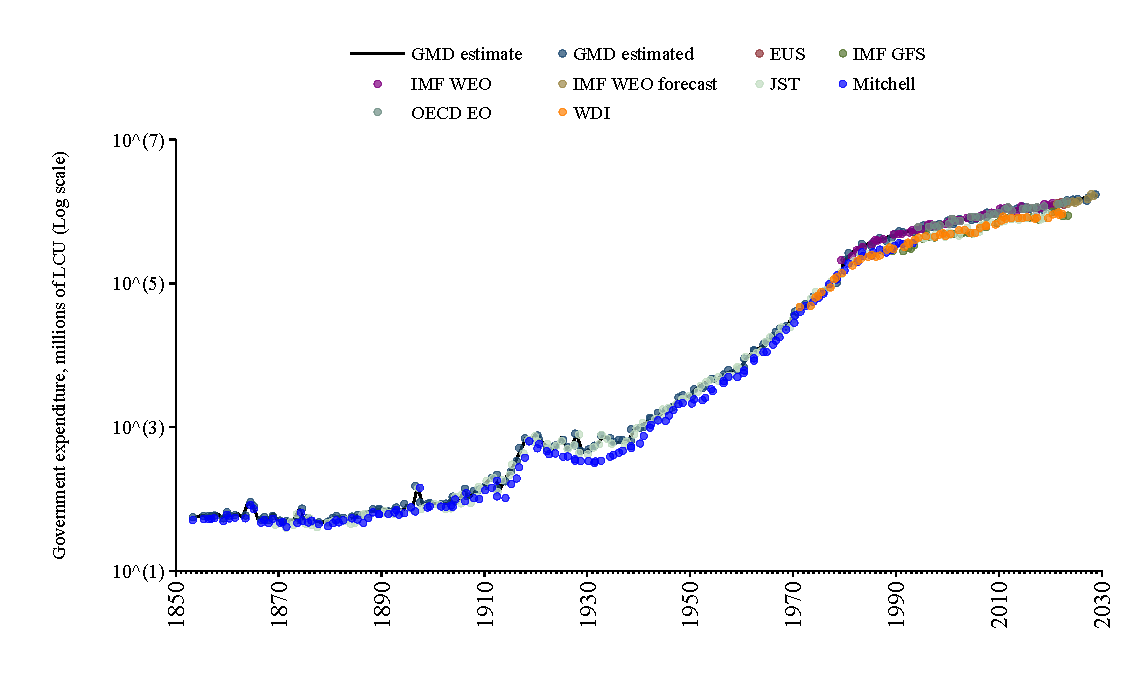
\includegraphics[width=\textwidth,height=0.6\textheight,keepaspectratio]{graphs/DNK_govexp.pdf}
\end{figure}
\end{minipage}
\end{adjustbox}
\begin{adjustbox}{max totalsize={\paperwidth}{\paperheight},center}
\begin{minipage}[t][\textheight][t]{\textwidth}
\vspace*{0.5cm}
\phantomsection
\addcontentsline{toc}{section}{Government expenditure to GDP ratio}
\begin{center}
{\Large\bfseries Government expenditure to GDP ratio}
\end{center}
\vspace{0.5cm}
\begin{table}[H]
\centering
\small
\begin{tabular}{|l|l|l|}
\hline
\textbf{Source} & \textbf{Time span} & \textbf{Notes} \\
\hline
\rowcolor{white}\cite{Mitchell}& 1854 - 1869 &Spliced using overlapping data in 1870. Data refers to central government.\\
\rowcolor{lightgray}\cite{JST}& 1870 - 1935 &Spliced using overlapping data in 1936. Data refers to central government.\\
\rowcolor{white}\cite{IMF_FPP}& 1936 - 1936 &Spliced using overlapping data in 1937. Data refers to general government.\\
\rowcolor{lightgray}\cite{JST}& 1937 - 1971 &Spliced using overlapping data in 1972. Data refers to central government.\\
\rowcolor{white}\cite{WDI}& 1972 - 1979 &Spliced using overlapping data in 1980. Data refers to general government.\\
\rowcolor{lightgray}\cite{IMF_WEO}& 1980 - 1994 &Spliced using overlapping data in 1995. Data refers to general government.\\
\rowcolor{white}\cite{EUS}& 1995 - 2024 &Baseline source, overlaps with base year 2018. Data refers to general government.\\
\rowcolor{lightgray}\cite{IMF_WEO_forecast}& 2025 - 2029 &Spliced using overlapping data in 2030. \\
\hline
\end{tabular}
\end{table}
\begin{figure}[H]
\centering
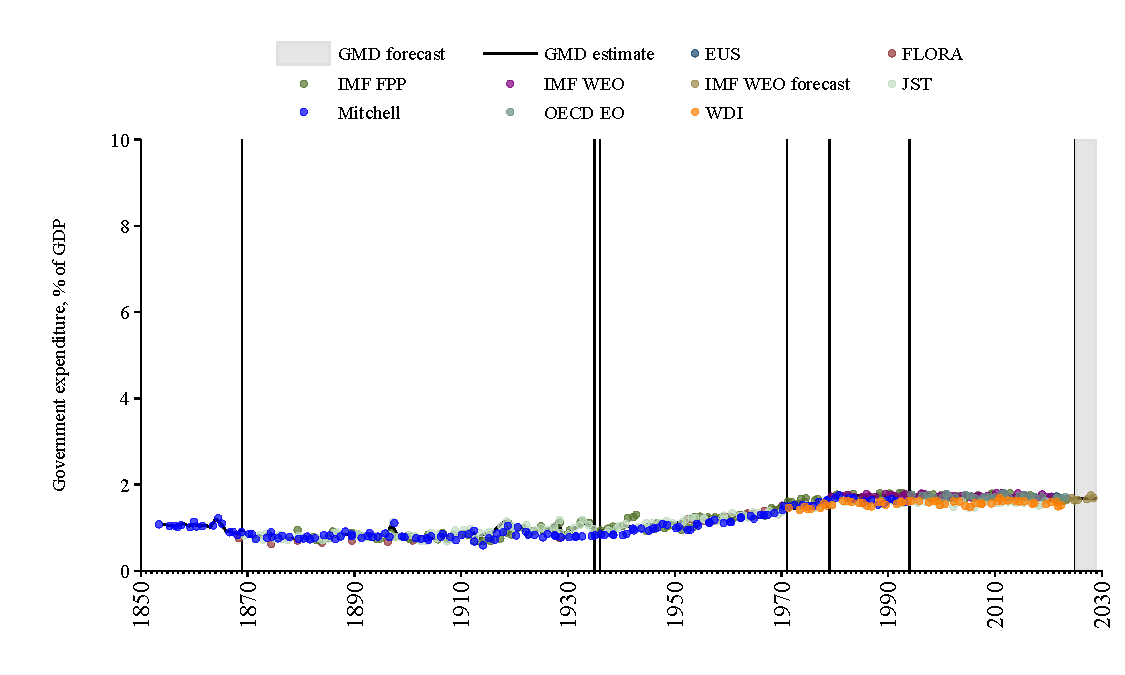
\includegraphics[width=\textwidth,height=0.6\textheight,keepaspectratio]{graphs/DNK_govexp_GDP.pdf}
\end{figure}
\end{minipage}
\end{adjustbox}
\begin{adjustbox}{max totalsize={\paperwidth}{\paperheight},center}
\begin{minipage}[t][\textheight][t]{\textwidth}
\vspace*{0.5cm}
\phantomsection
\addcontentsline{toc}{section}{Government revenue}
\begin{center}
{\Large\bfseries Government revenue}
\end{center}
\vspace{0.5cm}
\begin{table}[H]
\centering
\small
\begin{tabular}{|l|l|l|}
\hline
\textbf{Source} & \textbf{Time span} & \textbf{Notes} \\
\hline
\rowcolor{white}\cite{GMD_estimated}& 1853 - 2029 &Baseline source, overlaps with base year 2018. \\
\hline
\end{tabular}
\end{table}
\begin{figure}[H]
\centering
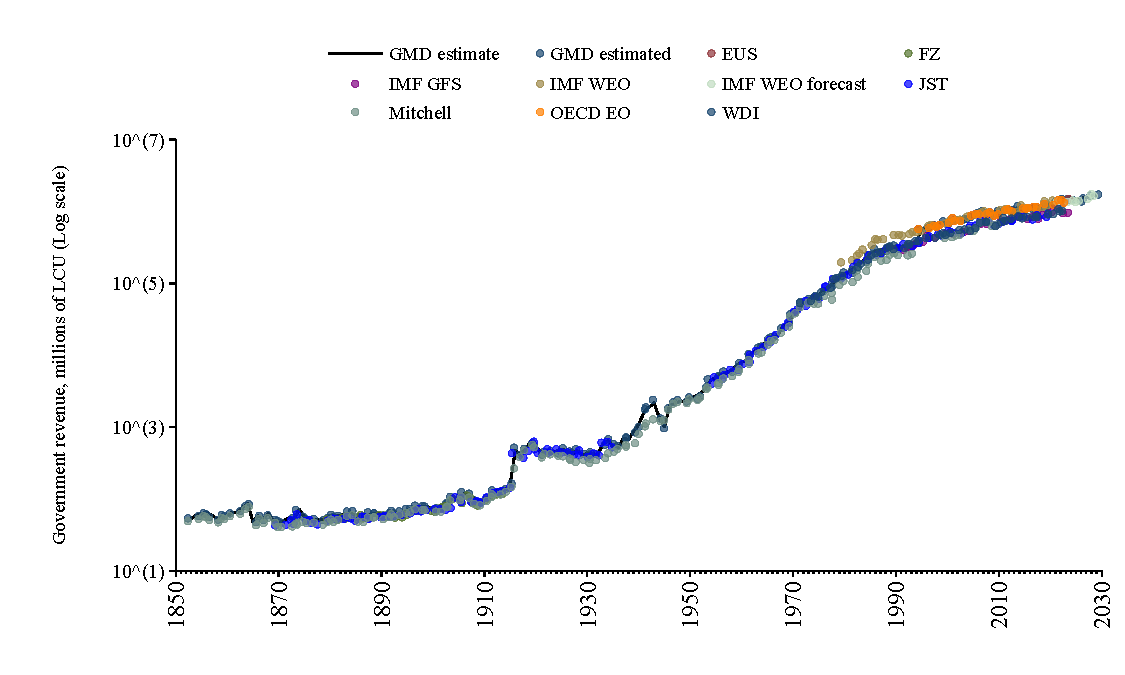
\includegraphics[width=\textwidth,height=0.6\textheight,keepaspectratio]{graphs/DNK_govrev.pdf}
\end{figure}
\end{minipage}
\end{adjustbox}
\begin{adjustbox}{max totalsize={\paperwidth}{\paperheight},center}
\begin{minipage}[t][\textheight][t]{\textwidth}
\vspace*{0.5cm}
\phantomsection
\addcontentsline{toc}{section}{Government revenue to GDP ratio}
\begin{center}
{\Large\bfseries Government revenue to GDP ratio}
\end{center}
\vspace{0.5cm}
\begin{table}[H]
\centering
\small
\begin{tabular}{|l|l|l|}
\hline
\textbf{Source} & \textbf{Time span} & \textbf{Notes} \\
\hline
\rowcolor{white}\cite{Mitchell}& 1853 - 1869 &Spliced using overlapping data in 1870. Data refers to central government.\\
\rowcolor{lightgray}\cite{JST}& 1870 - 1935 &Spliced using overlapping data in 1936. Data refers to central government.\\
\rowcolor{white}\cite{IMF_FPP}& 1936 - 1953 &Spliced using overlapping data in 1954. Data refers to general government.\\
\rowcolor{lightgray}\cite{JST}& 1954 - 1971 &Spliced using overlapping data in 1972. Data refers to central government.\\
\rowcolor{white}\cite{WDI}& 1972 - 1994 &Spliced using overlapping data in 1995. Data refers to general government.\\
\rowcolor{lightgray}\cite{OECD_EO}& 1995 - 2023 &Baseline source, overlaps with base year 2018. Data refers to general government.\\
\rowcolor{white}\cite{EUS}& 2024 - 2024 &Spliced using overlapping data in 2025. Data refers to general government.\\
\rowcolor{lightgray}\cite{IMF_WEO_forecast}& 2025 - 2029 &Spliced using overlapping data in 2030. \\
\hline
\end{tabular}
\end{table}
\begin{figure}[H]
\centering
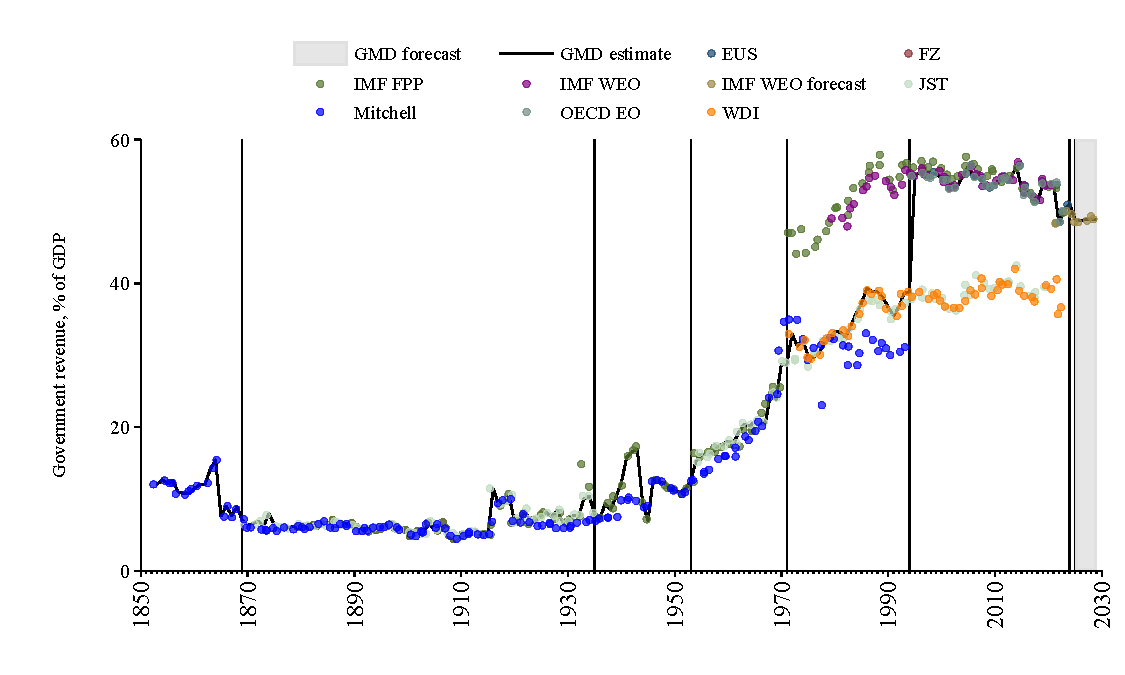
\includegraphics[width=\textwidth,height=0.6\textheight,keepaspectratio]{graphs/DNK_govrev_GDP.pdf}
\end{figure}
\end{minipage}
\end{adjustbox}
\begin{adjustbox}{max totalsize={\paperwidth}{\paperheight},center}
\begin{minipage}[t][\textheight][t]{\textwidth}
\vspace*{0.5cm}
\phantomsection
\addcontentsline{toc}{section}{Government tax revenue}
\begin{center}
{\Large\bfseries Government tax revenue}
\end{center}
\vspace{0.5cm}
\begin{table}[H]
\centering
\small
\begin{tabular}{|l|l|l|}
\hline
\textbf{Source} & \textbf{Time span} & \textbf{Notes} \\
\hline
\rowcolor{white}\cite{GMD_estimated}& 1853 - 2024 &Baseline source, overlaps with base year 2018. \\
\hline
\end{tabular}
\end{table}
\begin{figure}[H]
\centering
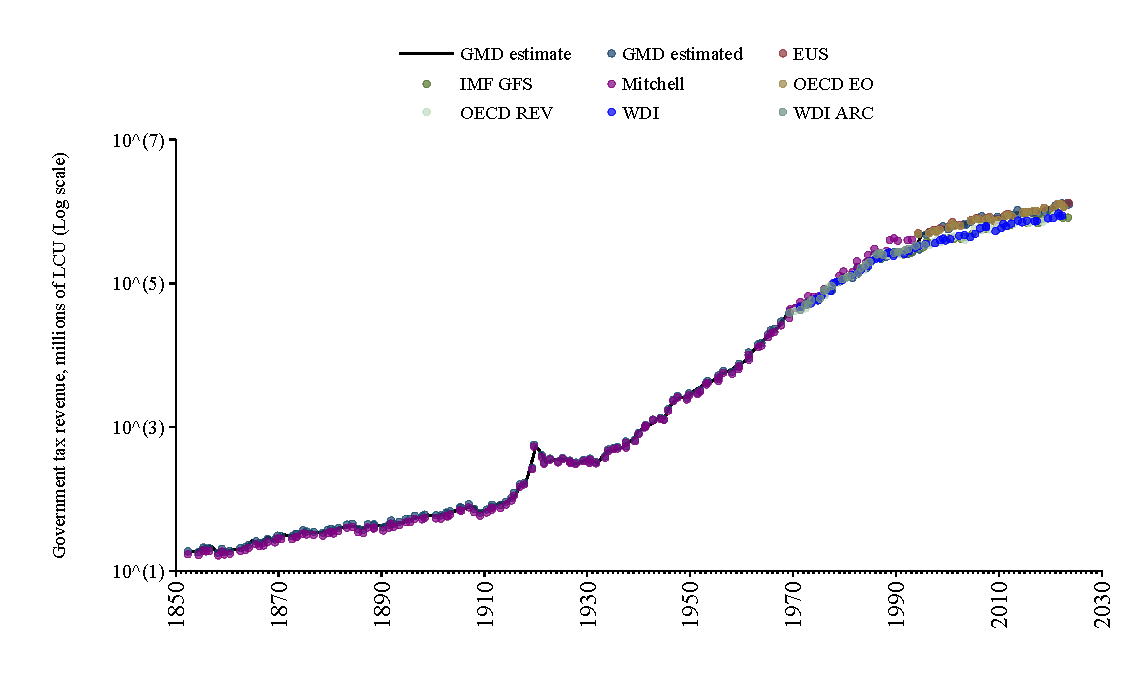
\includegraphics[width=\textwidth,height=0.6\textheight,keepaspectratio]{graphs/DNK_govtax.pdf}
\end{figure}
\end{minipage}
\end{adjustbox}
\begin{adjustbox}{max totalsize={\paperwidth}{\paperheight},center}
\begin{minipage}[t][\textheight][t]{\textwidth}
\vspace*{0.5cm}
\phantomsection
\addcontentsline{toc}{section}{Government tax revenue to GDP ratio}
\begin{center}
{\Large\bfseries Government tax revenue to GDP ratio}
\end{center}
\vspace{0.5cm}
\begin{table}[H]
\centering
\small
\begin{tabular}{|l|l|l|}
\hline
\textbf{Source} & \textbf{Time span} & \textbf{Notes} \\
\hline
\rowcolor{white}\cite{Mitchell}& 1853 - 1969 &Spliced using overlapping data in 1970. Data refers to central government.\\
\rowcolor{lightgray}\cite{WDI_ARC}& 1970 - 1971 &Spliced using overlapping data in 1972. Data refers to central government.\\
\rowcolor{white}\cite{WDI}& 1972 - 1994 &Spliced using overlapping data in 1995. Data refers to central government.\\
\rowcolor{lightgray}\cite{OECD_EO}& 1995 - 2023 &Baseline source, overlaps with base year 2018. Data refers to general government.\\
\rowcolor{white}\cite{EUS}& 2024 - 2024 &Spliced using overlapping data in 2025. Data refers to general government.\\
\hline
\end{tabular}
\end{table}
\begin{figure}[H]
\centering
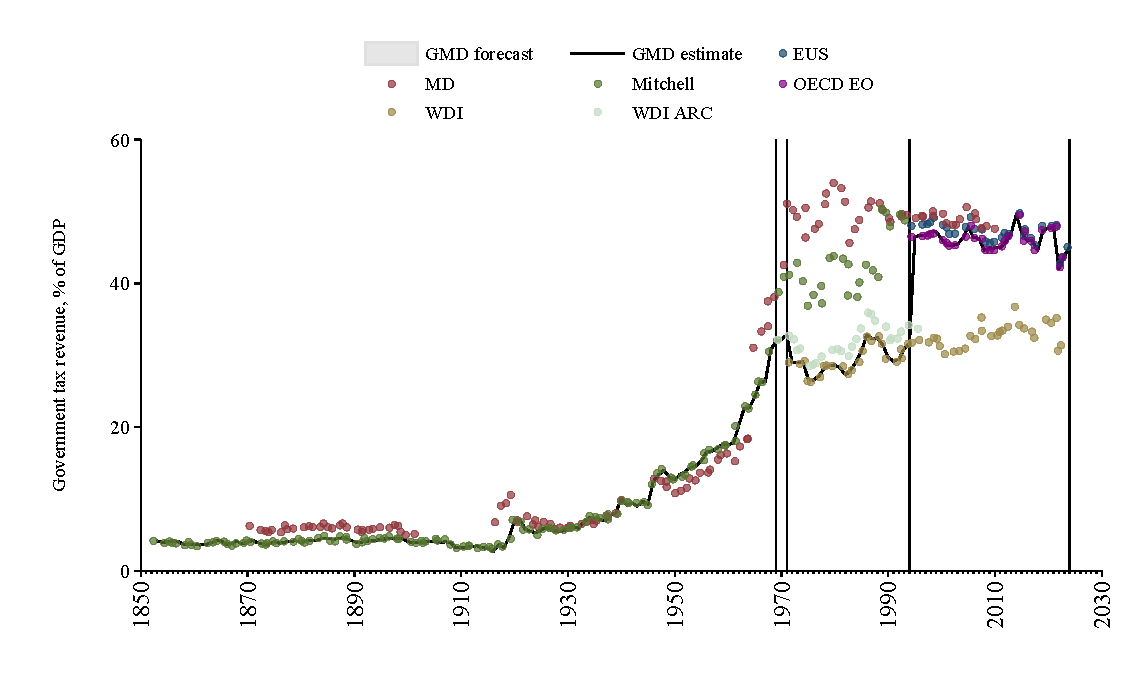
\includegraphics[width=\textwidth,height=0.6\textheight,keepaspectratio]{graphs/DNK_govtax_GDP.pdf}
\end{figure}
\end{minipage}
\end{adjustbox}
\begin{adjustbox}{max totalsize={\paperwidth}{\paperheight},center}
\begin{minipage}[t][\textheight][t]{\textwidth}
\vspace*{0.5cm}
\phantomsection
\addcontentsline{toc}{section}{Imports}
\begin{center}
{\Large\bfseries Imports}
\end{center}
\vspace{0.5cm}
\begin{table}[H]
\centering
\small
\begin{tabular}{|l|l|l|}
\hline
\textbf{Source} & \textbf{Time span} & \textbf{Notes} \\
\hline
\rowcolor{white}\cite{Tena}& 1841 - 1842 &Spliced using overlapping data in 1843: (ratio = 116.1\%). \\
\rowcolor{lightgray}\cite{CS1_DNK}& 1843 - 1959 &Spliced using overlapping data in 1960: (ratio = 100.6\%). \\
\rowcolor{white}\cite{AMECO}& 1960 - 1965 &Spliced using overlapping data in 1966: (ratio = 100.2\%). \\
\rowcolor{lightgray}\cite{OECD_EO}& 1966 - 2025 &Baseline source, overlaps with base year 2018. \\
\rowcolor{white}\cite{AMECO}& 2026 - 2026 &Spliced using overlapping data in 2027: (ratio = 101.2\%). \\
\rowcolor{lightgray}\cite{IMF_WEO_forecast}& 2027 - 2029 &Spliced using overlapping data in 2030: (ratio = 102.8\%). \\
\hline
\end{tabular}
\end{table}
\begin{figure}[H]
\centering
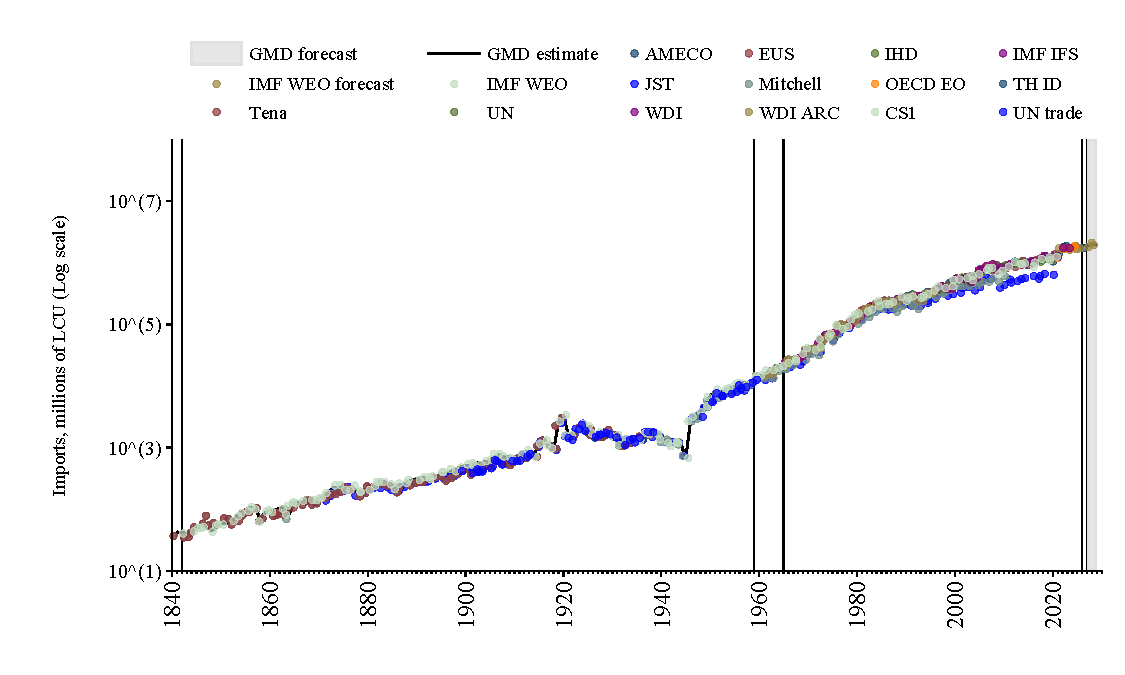
\includegraphics[width=\textwidth,height=0.6\textheight,keepaspectratio]{graphs/DNK_imports.pdf}
\end{figure}
\end{minipage}
\end{adjustbox}
\begin{adjustbox}{max totalsize={\paperwidth}{\paperheight},center}
\begin{minipage}[t][\textheight][t]{\textwidth}
\vspace*{0.5cm}
\phantomsection
\addcontentsline{toc}{section}{Imports to GDP ratio}
\begin{center}
{\Large\bfseries Imports to GDP ratio}
\end{center}
\vspace{0.5cm}
\begin{table}[H]
\centering
\small
\begin{tabular}{|l|l|l|}
\hline
\textbf{Source} & \textbf{Time span} & \textbf{Notes} \\
\hline
\rowcolor{white}\cite{Mitchell}& 1841 - 1842 &Spliced using overlapping data in 1843: (ratio = 102.9\%). \\
\rowcolor{lightgray}\cite{CS1_DNK}& 1843 - 1959 &Spliced using overlapping data in 1960: (ratio = 98\%). \\
\rowcolor{white}\cite{WDI_ARC}& 1960 - 1965 &Spliced using overlapping data in 1966: (ratio = 95.8\%). \\
\rowcolor{lightgray}\cite{OECD_EO}& 1966 - 2025 &Baseline source, overlaps with base year 2018. \\
\rowcolor{white}\cite{AMECO}& 2026 - 2026 &Spliced using overlapping data in 2027: (ratio = 102.7\%). \\
\rowcolor{lightgray}\cite{IMF_WEO_forecast}& 2027 - 2029 &Spliced using overlapping data in 2030: (ratio = 101\%). \\
\hline
\end{tabular}
\end{table}
\begin{figure}[H]
\centering
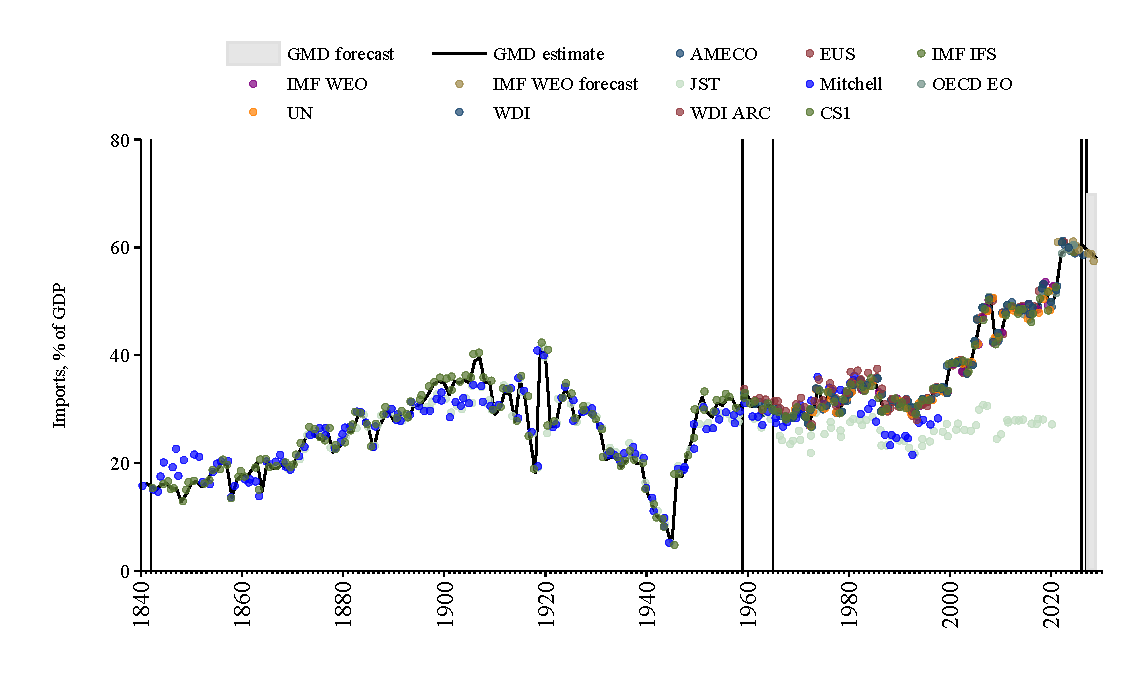
\includegraphics[width=\textwidth,height=0.6\textheight,keepaspectratio]{graphs/DNK_imports_GDP.pdf}
\end{figure}
\end{minipage}
\end{adjustbox}
\begin{adjustbox}{max totalsize={\paperwidth}{\paperheight},center}
\begin{minipage}[t][\textheight][t]{\textwidth}
\vspace*{0.5cm}
\phantomsection
\addcontentsline{toc}{section}{Inflation}
\begin{center}
{\Large\bfseries Inflation}
\end{center}
\vspace{0.5cm}
\begin{table}[H]
\centering
\small
\begin{tabular}{|l|l|l|}
\hline
\textbf{Source} & \textbf{Time span} & \textbf{Notes} \\
\hline
\rowcolor{white}\cite{CS1_DNK}& 1488 - 1900 &Spliced using overlapping data in 1901. \\
\rowcolor{lightgray}\cite{BIS}& 1901 - 1969 &Spliced using overlapping data in 1970. \\
\rowcolor{white}\cite{WB_CC}& 1970 - 2023 &Baseline source, overlaps with base year 2018. \\
\rowcolor{lightgray}\cite{BIS}& 2024 - 2024 &Spliced using overlapping data in 2025. \\
\rowcolor{white}\cite{IMF_WEO_forecast}& 2025 - 2029 &Spliced using overlapping data in 2030. \\
\hline
\end{tabular}
\end{table}
\begin{figure}[H]
\centering
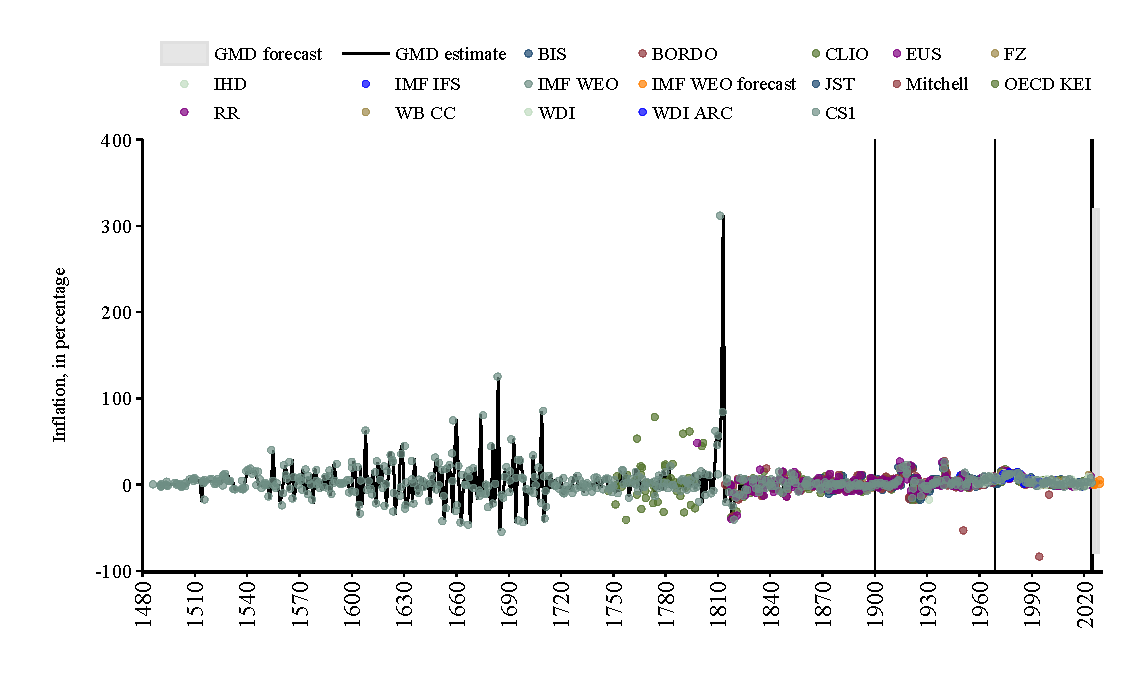
\includegraphics[width=\textwidth,height=0.6\textheight,keepaspectratio]{graphs/DNK_infl.pdf}
\end{figure}
\end{minipage}
\end{adjustbox}
\begin{adjustbox}{max totalsize={\paperwidth}{\paperheight},center}
\begin{minipage}[t][\textheight][t]{\textwidth}
\vspace*{0.5cm}
\phantomsection
\addcontentsline{toc}{section}{Investment}
\begin{center}
{\Large\bfseries Investment}
\end{center}
\vspace{0.5cm}
\begin{table}[H]
\centering
\small
\begin{tabular}{|l|l|l|}
\hline
\textbf{Source} & \textbf{Time span} & \textbf{Notes} \\
\hline
\rowcolor{white}\cite{CS1_DNK}& 1835 - 1959 &Spliced using overlapping data in 1960: (ratio = 102.4\%). \\
\rowcolor{lightgray}\cite{AMECO}& 1960 - 1965 &Spliced using overlapping data in 1966. \\
\rowcolor{white}\cite{OECD_EO}& 1966 - 2025 &Baseline source, overlaps with base year 2018. \\
\rowcolor{lightgray}\cite{AMECO}& 2026 - 2026 &Spliced using overlapping data in 2027: (ratio = 88.3\%). \\
\rowcolor{white}\cite{IMF_WEO_forecast}& 2027 - 2029 &Spliced using overlapping data in 2030: (ratio = 95.4\%). \\
\hline
\end{tabular}
\end{table}
\begin{figure}[H]
\centering
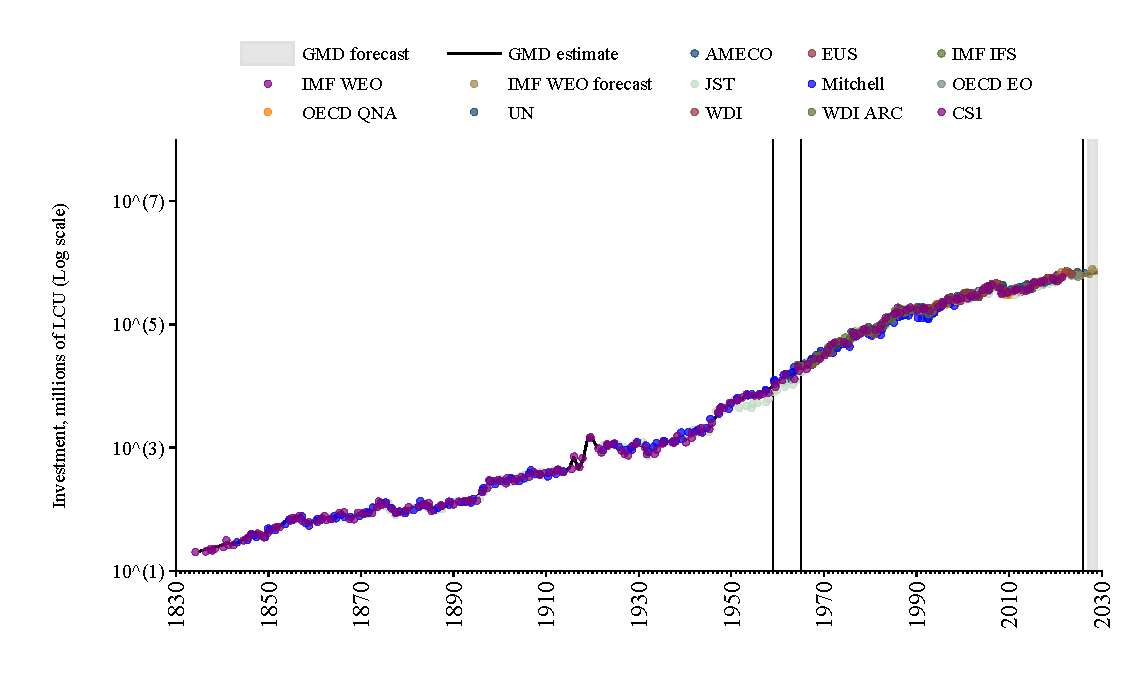
\includegraphics[width=\textwidth,height=0.6\textheight,keepaspectratio]{graphs/DNK_inv.pdf}
\end{figure}
\end{minipage}
\end{adjustbox}
\begin{adjustbox}{max totalsize={\paperwidth}{\paperheight},center}
\begin{minipage}[t][\textheight][t]{\textwidth}
\vspace*{0.5cm}
\phantomsection
\addcontentsline{toc}{section}{Investment to GDP ratio}
\begin{center}
{\Large\bfseries Investment to GDP ratio}
\end{center}
\vspace{0.5cm}
\begin{table}[H]
\centering
\small
\begin{tabular}{|l|l|l|}
\hline
\textbf{Source} & \textbf{Time span} & \textbf{Notes} \\
\hline
\rowcolor{white}\cite{CS1_DNK}& 1835 - 1959 &Spliced using overlapping data in 1960: (ratio = 102\%). \\
\rowcolor{lightgray}\cite{AMECO}& 1960 - 1964 &Spliced using overlapping data in 1965. \\
\rowcolor{white}\cite{WDI_ARC}& 1965 - 1965 &Spliced using overlapping data in 1966: (ratio = 89.3\%). \\
\rowcolor{lightgray}\cite{OECD_EO}& 1966 - 2025 &Baseline source, overlaps with base year 2018. \\
\rowcolor{white}\cite{AMECO}& 2026 - 2026 &Spliced using overlapping data in 2027: (ratio = 89.6\%). \\
\rowcolor{lightgray}\cite{IMF_WEO_forecast}& 2027 - 2029 &Spliced using overlapping data in 2030: (ratio = 93.7\%). \\
\hline
\end{tabular}
\end{table}
\begin{figure}[H]
\centering
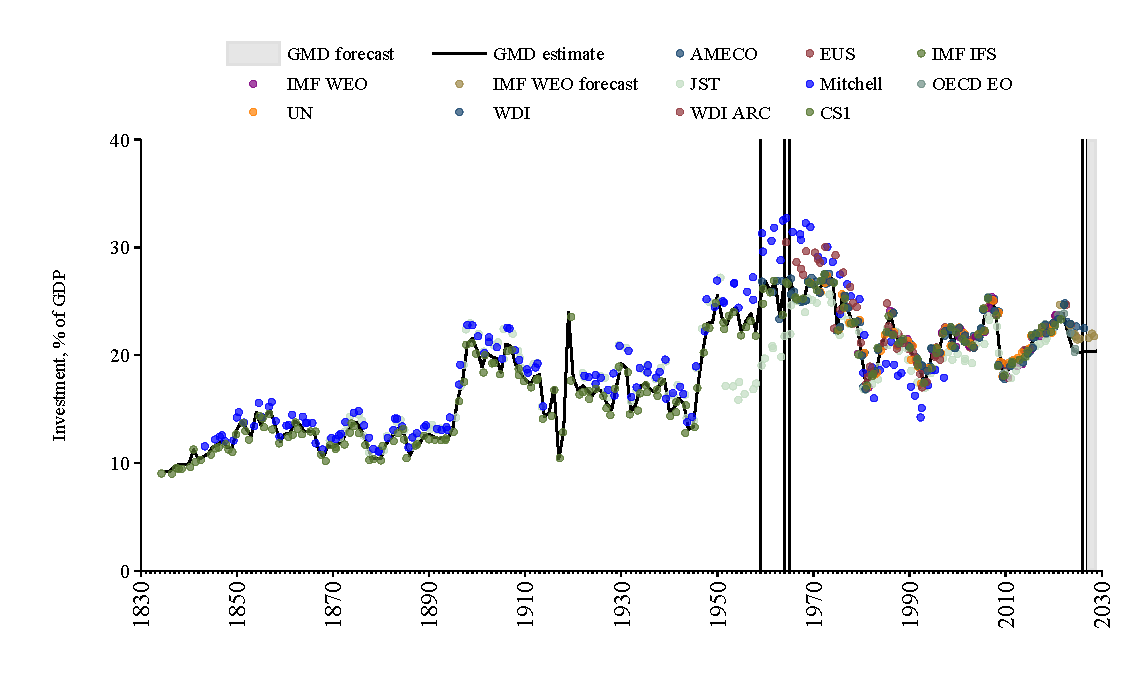
\includegraphics[width=\textwidth,height=0.6\textheight,keepaspectratio]{graphs/DNK_inv_GDP.pdf}
\end{figure}
\end{minipage}
\end{adjustbox}
\begin{adjustbox}{max totalsize={\paperwidth}{\paperheight},center}
\begin{minipage}[t][\textheight][t]{\textwidth}
\vspace*{0.5cm}
\phantomsection
\addcontentsline{toc}{section}{Long term interest rate}
\begin{center}
{\Large\bfseries Long term interest rate}
\end{center}
\vspace{0.5cm}
\begin{table}[H]
\centering
\small
\begin{tabular}{|l|l|l|}
\hline
\textbf{Source} & \textbf{Time span} & \textbf{Notes} \\
\hline
\rowcolor{white}\cite{CS1_DNK}& 1814 - 1869 &Spliced using overlapping data in 1870. \\
\rowcolor{lightgray}\cite{JST}& 1870 - 1954 &Spliced using overlapping data in 1955. \\
\rowcolor{white}\cite{OECD_MEI_ARC}& 1955 - 1984 &Spliced using overlapping data in 1985. \\
\rowcolor{lightgray}\cite{EUS}& 1985 - 1986 &Spliced using overlapping data in 1987. \\
\rowcolor{white}\cite{OECD_MEI}& 1987 - 2023 &Baseline source, overlaps with base year 2018. \\
\rowcolor{lightgray}\cite{EUS}& 2024 - 2024 &Spliced using overlapping data in 2025. \\
\hline
\end{tabular}
\end{table}
\begin{figure}[H]
\centering
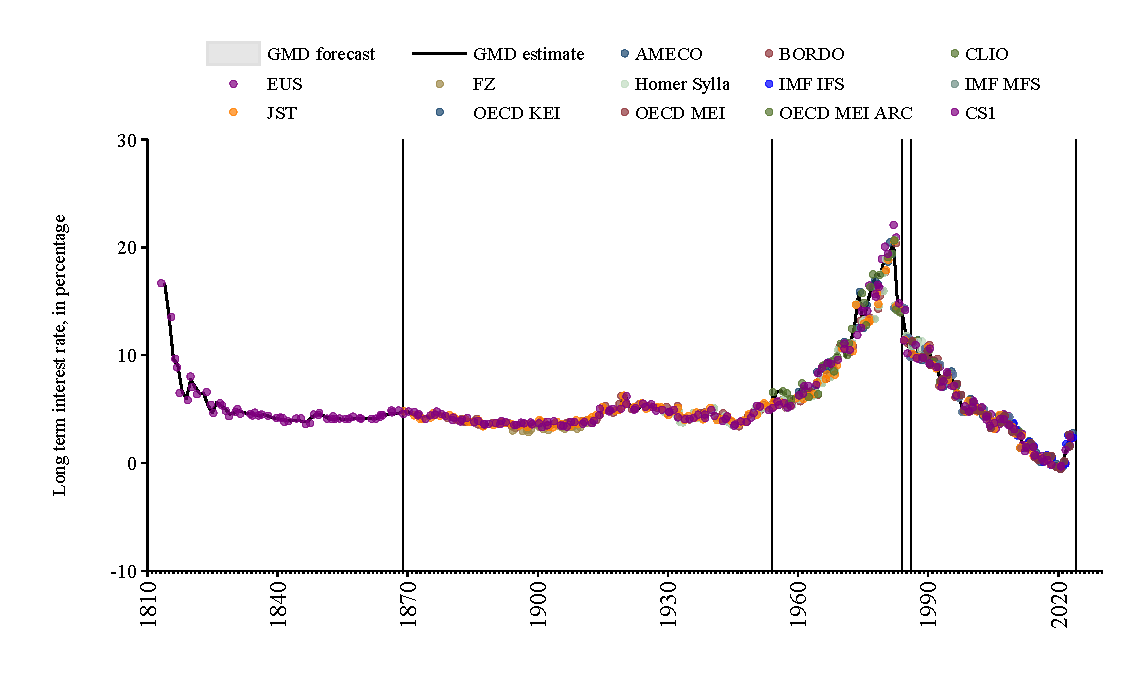
\includegraphics[width=\textwidth,height=0.6\textheight,keepaspectratio]{graphs/DNK_ltrate.pdf}
\end{figure}
\end{minipage}
\end{adjustbox}
\begin{adjustbox}{max totalsize={\paperwidth}{\paperheight},center}
\begin{minipage}[t][\textheight][t]{\textwidth}
\vspace*{0.5cm}
\phantomsection
\addcontentsline{toc}{section}{Nominal GDP}
\begin{center}
{\Large\bfseries Nominal GDP}
\end{center}
\vspace{0.5cm}
\begin{table}[H]
\centering
\small
\begin{tabular}{|l|l|l|}
\hline
\textbf{Source} & \textbf{Time span} & \textbf{Notes} \\
\hline
\rowcolor{white}\cite{CS1_DNK}& 1815 - 1949 &Spliced using overlapping data in 1950: (ratio = 100.7\%). \\
\rowcolor{lightgray}\cite{IMF_GDD}& 1950 - 1959 &Spliced using overlapping data in 1960: (ratio = 100.8\%). \\
\rowcolor{white}\cite{AMECO}& 1960 - 1965 &Spliced using overlapping data in 1966. \\
\rowcolor{lightgray}\cite{OECD_EO}& 1966 - 2025 &Baseline source, overlaps with base year 2018. \\
\rowcolor{white}\cite{AMECO}& 2026 - 2026 &Spliced using overlapping data in 2027: (ratio = 98.6\%). \\
\rowcolor{lightgray}\cite{IMF_WEO_forecast}& 2027 - 2029 &Spliced using overlapping data in 2030: (ratio = 101.9\%). \\
\hline
\end{tabular}
\end{table}
\begin{figure}[H]
\centering
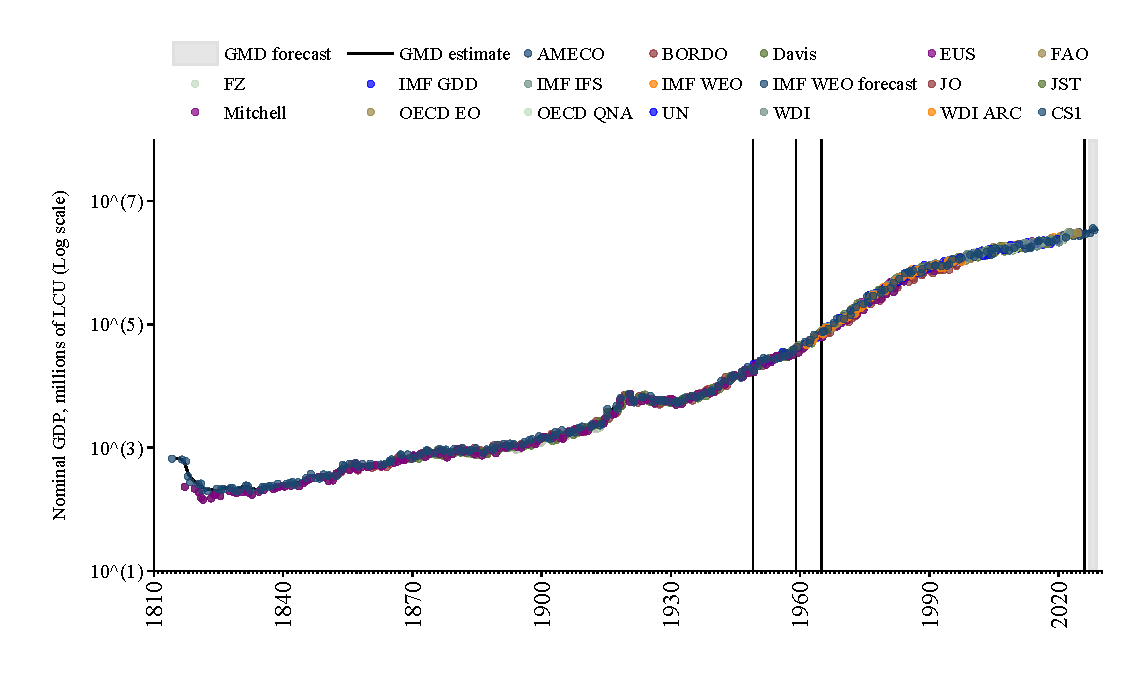
\includegraphics[width=\textwidth,height=0.6\textheight,keepaspectratio]{graphs/DNK_nGDP.pdf}
\end{figure}
\end{minipage}
\end{adjustbox}
\begin{adjustbox}{max totalsize={\paperwidth}{\paperheight},center}
\begin{minipage}[t][\textheight][t]{\textwidth}
\vspace*{0.5cm}
\phantomsection
\addcontentsline{toc}{section}{Population}
\begin{center}
{\Large\bfseries Population}
\end{center}
\vspace{0.5cm}
\begin{table}[H]
\centering
\small
\begin{tabular}{|l|l|l|}
\hline
\textbf{Source} & \textbf{Time span} & \textbf{Notes} \\
\hline
\rowcolor{white}\cite{CS1_DNK}& 1735 - 1949 &Spliced using overlapping data in 1950: (ratio = 99.8\%). \\
\rowcolor{lightgray}\cite{IMF_IFS}& 1950 - 1959 &Spliced using overlapping data in 1960. \\
\rowcolor{white}\cite{WDI}& 1960 - 2023 &Baseline source, overlaps with base year 2018. \\
\rowcolor{lightgray}\cite{OECD_EO}& 2024 - 2025 &Spliced using overlapping data in 2026: (ratio = 100.1\%). \\
\rowcolor{white}\cite{AMECO}& 2026 - 2026 &Spliced using overlapping data in 2027: (ratio = 99.9\%). \\
\rowcolor{lightgray}\cite{Gapminder}& 2027 - 2030 &Spliced using overlapping data in 2031. \\
\hline
\end{tabular}
\end{table}
\begin{figure}[H]
\centering
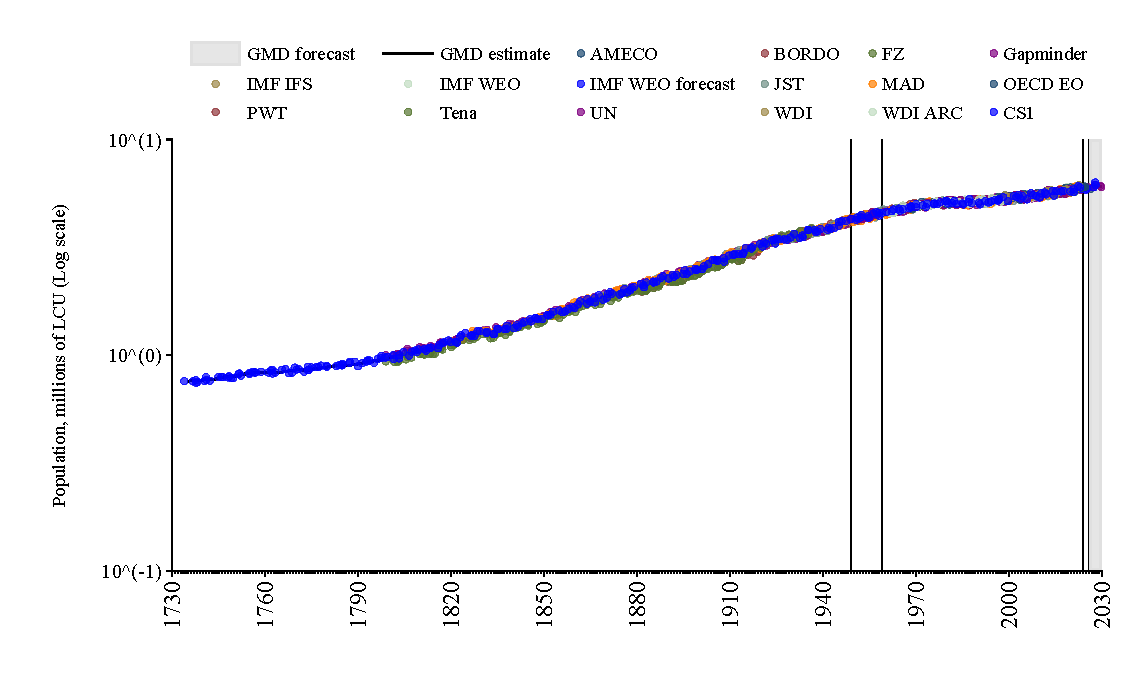
\includegraphics[width=\textwidth,height=0.6\textheight,keepaspectratio]{graphs/DNK_pop.pdf}
\end{figure}
\end{minipage}
\end{adjustbox}
\begin{adjustbox}{max totalsize={\paperwidth}{\paperheight},center}
\begin{minipage}[t][\textheight][t]{\textwidth}
\vspace*{0.5cm}
\phantomsection
\addcontentsline{toc}{section}{Real GDP}
\begin{center}
{\Large\bfseries Real GDP}
\end{center}
\vspace{0.5cm}
\begin{table}[H]
\centering
\small
\begin{tabular}{|l|l|l|}
\hline
\textbf{Source} & \textbf{Time span} & \textbf{Notes} \\
\hline
\rowcolor{white}\cite{CS1_DNK}& 1815 - 1959 &Spliced using overlapping data in 1960: (ratio = 101.6\%). \\
\rowcolor{lightgray}\cite{AMECO}& 1960 - 1965 &Spliced using overlapping data in 1966: (ratio = 103.3\%). \\
\rowcolor{white}\cite{OECD_EO}& 1966 - 2025 &Baseline source, overlaps with base year 2018. \\
\rowcolor{lightgray}\cite{AMECO}& 2026 - 2026 &Spliced using overlapping data in 2027: (ratio = 98.5\%). \\
\rowcolor{white}\cite{IMF_WEO_forecast}& 2027 - 2029 &Spliced using overlapping data in 2030: (ratio = 100.1\%). \\
\hline
\end{tabular}
\end{table}
\begin{figure}[H]
\centering
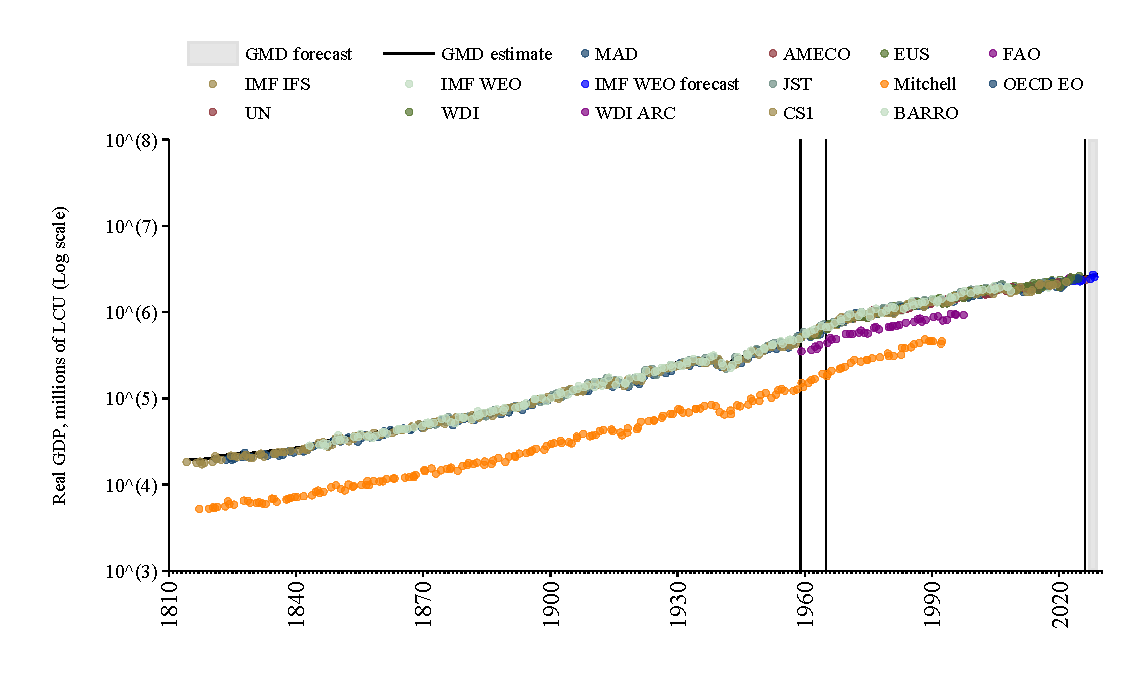
\includegraphics[width=\textwidth,height=0.6\textheight,keepaspectratio]{graphs/DNK_rGDP.pdf}
\end{figure}
\end{minipage}
\end{adjustbox}
\begin{adjustbox}{max totalsize={\paperwidth}{\paperheight},center}
\begin{minipage}[t][\textheight][t]{\textwidth}
\vspace*{0.5cm}
\phantomsection
\addcontentsline{toc}{section}{Real total consumption}
\begin{center}
{\Large\bfseries Real total consumption}
\end{center}
\vspace{0.5cm}
\begin{table}[H]
\centering
\small
\begin{tabular}{|l|l|l|}
\hline
\textbf{Source} & \textbf{Time span} & \textbf{Notes} \\
\hline
\rowcolor{white}\cite{BARRO}& 1844 - 1965 &Spliced using overlapping data in 1966. \\
\rowcolor{lightgray}\cite{IMF_IFS}& 1966 - 2024 &Baseline source, overlaps with base year 2018. \\
\hline
\end{tabular}
\end{table}
\begin{figure}[H]
\centering
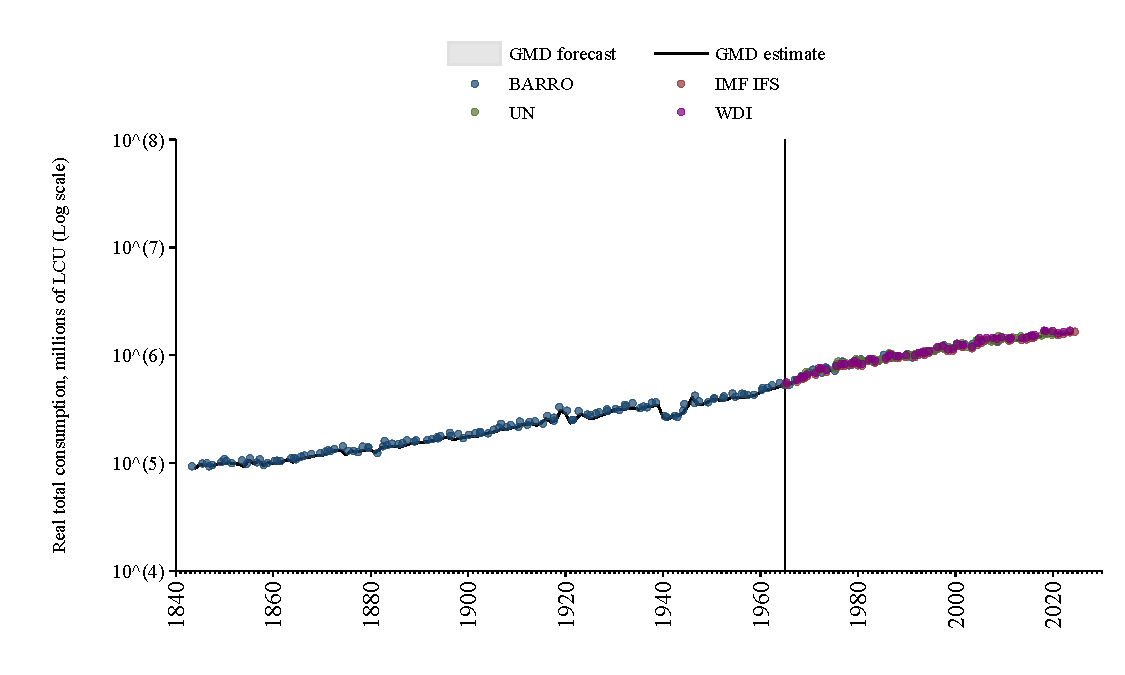
\includegraphics[width=\textwidth,height=0.6\textheight,keepaspectratio]{graphs/DNK_rcons.pdf}
\end{figure}
\end{minipage}
\end{adjustbox}
\begin{adjustbox}{max totalsize={\paperwidth}{\paperheight},center}
\begin{minipage}[t][\textheight][t]{\textwidth}
\vspace*{0.5cm}
\phantomsection
\addcontentsline{toc}{section}{Short term interest rate}
\begin{center}
{\Large\bfseries Short term interest rate}
\end{center}
\vspace{0.5cm}
\begin{table}[H]
\centering
\small
\begin{tabular}{|l|l|l|}
\hline
\textbf{Source} & \textbf{Time span} & \textbf{Notes} \\
\hline
\rowcolor{white}\cite{JST}& 1875 - 1960 &Spliced using overlapping data in 1961. \\
\rowcolor{lightgray}\cite{AMECO}& 1961 - 1979 &Spliced using overlapping data in 1980. \\
\rowcolor{white}\cite{OECD_EO}& 1980 - 1986 &Spliced using overlapping data in 1987. \\
\rowcolor{lightgray}\cite{OECD_KEI}& 1987 - 2023 &Baseline source, overlaps with base year 2018. \\
\rowcolor{white}\cite{OECD_EO}& 2024 - 2025 &Spliced using overlapping data in 2026. \\
\hline
\end{tabular}
\end{table}
\begin{figure}[H]
\centering
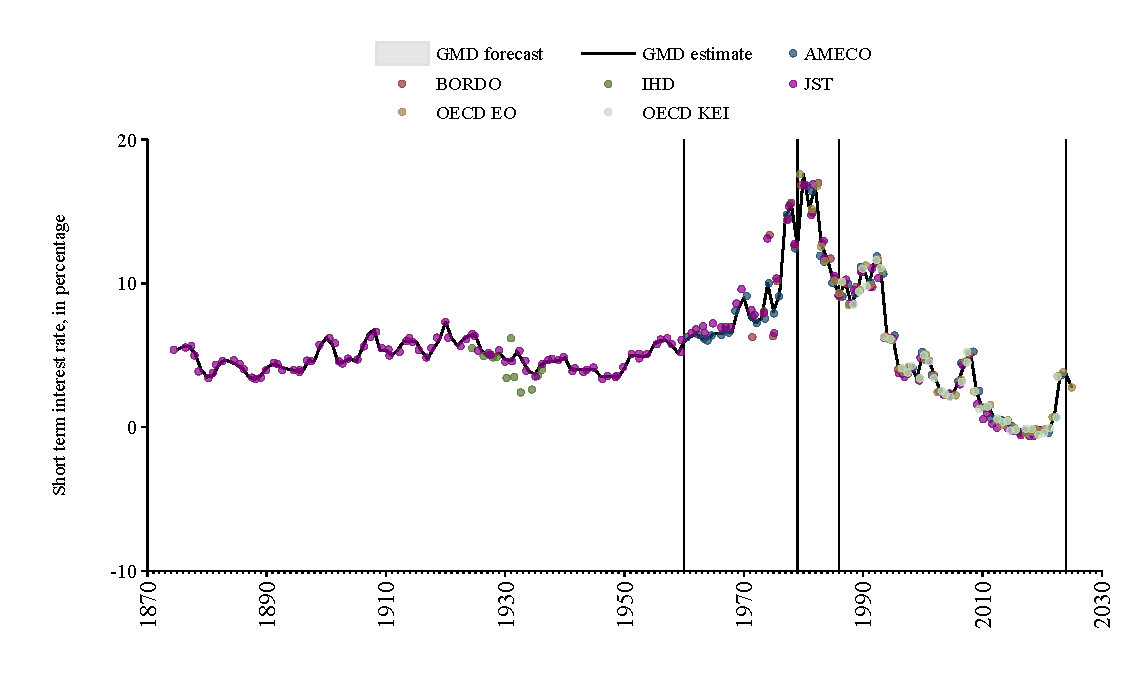
\includegraphics[width=\textwidth,height=0.6\textheight,keepaspectratio]{graphs/DNK_strate.pdf}
\end{figure}
\end{minipage}
\end{adjustbox}
\begin{adjustbox}{max totalsize={\paperwidth}{\paperheight},center}
\begin{minipage}[t][\textheight][t]{\textwidth}
\vspace*{0.5cm}
\phantomsection
\addcontentsline{toc}{section}{Unemployment}
\begin{center}
{\Large\bfseries Unemployment}
\end{center}
\vspace{0.5cm}
\begin{table}[H]
\centering
\small
\begin{tabular}{|l|l|l|}
\hline
\textbf{Source} & \textbf{Time span} & \textbf{Notes} \\
\hline
\rowcolor{white}\cite{JST}& 1874 - 1899 &Spliced using overlapping data in 1900. \\
\rowcolor{lightgray}\cite{CS1_DNK}& 1900 - 1959 &Spliced using overlapping data in 1960. \\
\rowcolor{white}\cite{AMECO}& 1960 - 1968 &Spliced using overlapping data in 1969. \\
\rowcolor{lightgray}\cite{OECD_EO}& 1969 - 2008 &Spliced using overlapping data in 2009. \\
\rowcolor{white}\cite{EUS}& 2009 - 2024 &Baseline source, overlaps with base year 2018. \\
\rowcolor{lightgray}\cite{OECD_EO}& 2025 - 2025 &Spliced using overlapping data in 2026. \\
\rowcolor{white}\cite{AMECO}& 2026 - 2026 &Spliced using overlapping data in 2027. \\
\rowcolor{lightgray}\cite{IMF_WEO_forecast}& 2027 - 2029 &Spliced using overlapping data in 2030. \\
\hline
\end{tabular}
\end{table}
\begin{figure}[H]
\centering
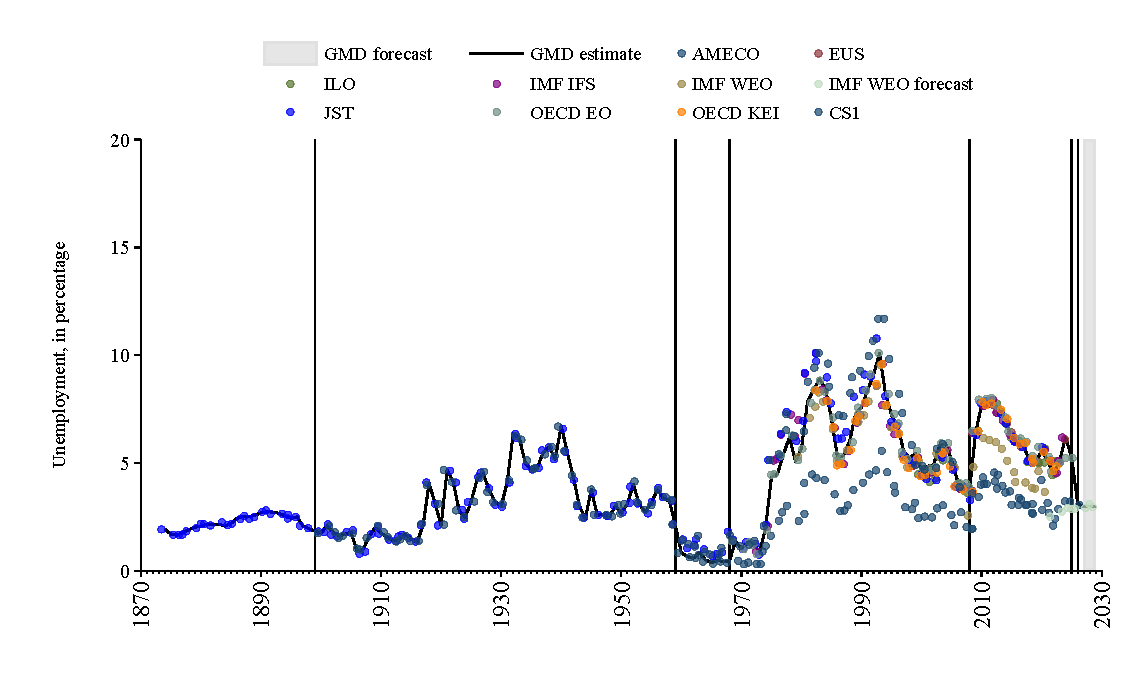
\includegraphics[width=\textwidth,height=0.6\textheight,keepaspectratio]{graphs/DNK_unemp.pdf}
\end{figure}
\end{minipage}
\end{adjustbox}
\phantomsection
\addcontentsline{toc}{section}{References}
\begin{center}
{\Large\bfseries References}
\end{center}
\small
\bibliographystyle{qje}
\bibliography{bib}
\end{document}
